% !TEX program = XeLaTex
\documentclass[12pt]{book}

% ----------------------------------------------------------------
% -- PACKAGES -- %
% ----------------------------------------------------------------
% Import graphics.
\usepackage{graphicx}

% Page settings.
\usepackage[margin = 1.2in, showframe]{geometry}

% LaTeX figure placing.
\usepackage{subcaption}
\usepackage{float}

% Special tables.
\usepackage{longtable}
\usepackage{chngpage}

\usepackage{enumitem}

\usepackage{amsmath, amsthm, amssymb}
\usepackage{mathrsfs}

% Figures and plotting.
\usepackage{pstricks}
\usepackage{multido}
\usepackage{pst-plot}

% Fonts.
\usepackage{fontspec}

% Titling.
\usepackage{titling}
\renewcommand\maketitlehooka{\null\mbox{}\vfill}
\renewcommand\maketitlehookd{\vfill\null}

% Headers.
% \usepackage{fancyhdr}


% Links.
\usepackage[colorlinks = true]{hyperref}

% ---------------------------------------------------------------- %
% -- FONTS -- %
% ---------------------------------------------------------------- %
\usepackage[T1]{fontenc}
% \usepackage[bitstream-charter]{mathdesign}
\setmainfont{ACaslonPro-Regular}
\defaultfontfeatures{
    Path = ~/Library/Fonts/,
    Extension = .otf,
    UprightFont = *-Regular,
    BoldFont = *-Bold,
    ItalicFont = *-Italic,
    BoldItalicFont = *-BoldItalic,
}
  
% ---------------------------------------------------------------- %
% -- TITLING -- %
% ---------------------------------------------------------------- %
\title
{   
    % \begin{center}
    %     \includegraphics[width = 40mm]{Images/LOGON.eps}
    % \end{center}
    \vspace{-50pt}
    \huge \textbf{N O T E S\;\;I N\;\;M A T H E M A T I C S}
}
\author{Anirudh Bhashyam}
\date{}

% ---------------------------------------------------------------- %
% -- HEADERS -- %
% ---------------------------------------------------------------- %
% \pagestyle{fancy}
% \fancyhf{}
% \rhead{\small Neer Treatment Solutions Pvt. Ltd\\
% \small Email: contactus@neerglobal.com\\
% \small CIN: U74999DL2020PTC362727}
% \lhead{\includegraphics[width = 20mm]{Images/12.eps}}
% \rfoot{\thepage}

% ---------------------------------------------------------------- %
% --- COMMANDS --- %
% ---------------------------------------------------------------- %

% -- Theorem Environment Settings -- %
\definecolor{thmcolor}{RGB}{142, 50, 1}
\newtheoremstyle{thmstyle}{}{}{\color{thmcolor}}{}{\color{thmcolor}\bfseries}{}{ }{}
\theoremstyle{thmstyle}
\newtheorem{thm}{Theorem}[section]

% -- Proof Environment Settings -- %
\definecolor{proofcolor}{RGB}{209, 134, 6}
\let\oldproof\proof
\renewcommand{\proof}{\color{proofcolor}\oldproof}

% -- Defintion Environment Settings -- %
\definecolor{defncolor}{RGB}{23, 20, 119}
\newtheoremstyle{defnstyle}{}{}{\color{defncolor}}{}{\color{defncolor}\bfseries}{}{ }{}
\theoremstyle{defnstyle}
\newtheorem{defn}[thm]{Definition}
\newcommand{\defnref}[1]{{\color{defncolor} Defintion #1}}

%  -- Example Environment Settings -- %
\definecolor{exmpcolor}{RGB}{0, 112, 72}
\newtheoremstyle{exmpstyle}{}{}{\color{exmpcolor}}{}{\color{exmpcolor}\bfseries}{}{ }{}
\theoremstyle{exmpstyle}
\newtheorem{exmp}{Example}[section]
\newcommand{\exmpref}[1]{{\color{exmpcolor} Example #1}}

%  -- Math Commands -- %
\newcommand{\norm}[1]{\left\lVert #1 \right\rVert}
\newcommand{\innerprod}[2]{\left\langle #1,\;#2 \right\rangle}
\newcommand{\abs}[1]{\left\lvert #1 \right\rvert}
\DeclareMathOperator*{\argmax}{argmax}
\DeclareMathOperator*{\argmin}{argmin}

% -- Dirac Notation -- %
\newcommand{\bra}[1]{\left\langle #1 \right\rvert}
\newcommand{\ket}[1]{\left\lvert #1 \right\rangle}
\newcommand{\braket}[2]{\left\langle #1 \vert #2 \right\rangle}
\newcommand{\ketbra}[2]{\left\lvert #1 \times #2 \right\rvert}

% -- Circuits -- %
\newcommand{\hadamardn}[1]{H^{\otimes #1}}

\newenvironment{amatrix}[1]{%
  \left(\begin{array}{@{}*{#1}{c}|c@{}}
}{%
  \end{array}\right)
}


% ---------------------------------------------------------------- %
% --- PSTRICKS OBJECTS --- %
% ---------------------------------------------------------------- %




\bibliography{./literature/refs.bib}

\begin{document}
    \begin{titlingpage}
        \maketitle
        \vspace{-50pt}
        \begin{center}
            \Large C O M P L E X\;\;A N A L Y S I S 
        \end{center}
    \end{titlingpage}

\tableofcontents

\chapter{Complex Numbers}
\section{Roots of Complex Numbers}
It is an interesting question to ask as to what the $n-$th roots of complex numbers are. After all, the basis of definition of the complex numbers is that they are numbers that can be expressed as a sum of real and imaginary parts. With the imaginary part being constituted of $i = \sqrt{-1}.$ To understand the notion of such roots we must define what it means for complex numbers to be equal (in the sense of their polar notation). In standard notation, it would boil down to the fact that the real and imaginary parts of a complex number are equal.

\begin{defn}[Equality of Complex Numbers]
    Two complex numbers $z_1 = r_1e^{i\theta_{1}}$ and $z_2 = r_2e^{i\theta_{2}}$ are equal if and only if $r_1 = r_2$ and $\theta_{1} = \theta_{2} + 2\pi k$, where $k \in \mathbb{Z}$.
\end{defn}

That is to say, in the Argand (complex) plane, going around by a multiple of $2\pi$, provided that $r$ stays the same, yields the same complex number. This simple principle can be used to express what we are trying to delineate. Suppose, we wish to find $z = r e^{i\theta} \in \mathbb{C}$ such that it is the answer to the expression $\sqrt[n]{r_0 e^{i\theta_{0}}}.$ In other words,
\[
    (r e^{i\theta})^{n} = r_0 e^{i\theta_{0}}.
\]  
Since, we know when complex numbers are equal, we can say that the expression above leads to the conclusion that (using \textit{De Moivre's theorem})
\[
    r^{n} = r\;\;\text{and}\;\; n\theta = \theta_{0} + 2\pi k,
\]
where $k \in \mathbb{Z}.$ This permits us to write the root $z$ as 
\[
    z = \sqrt[n]{r_0} e^{i\left(\frac{\theta_{0}}{n} + \frac{2\pi k}{n}\right)}.
\]
If we are to be precise, after $k \geq n$, the expression $(2\pi k) / n$ will reduce to a form $(2 \pi k') /n,$ where $k' \in \mathbb{Z}^{+}_{n}.$ Which reduces the number of possible roots to $n$, which agrees with the \textit{Fundamental Theorem of Algebra}. Since, we are restricted to the integers when using \textit{De Moivre's theorem}, we require other tools to make meaningful assumptions about complex powers, which we will see later.

\begin{exmp}
    $(-8i)^{1/3}.$
\end{exmp}
\begin{align*}
    (-8i)^{1/3} 
        &=
            (8e^{i(-\pi/2)})^{1/3} \\
        &=
            2 e^{i\left(-\frac{\pi}{6} + \frac{2\pi k}{3}\right)},
\end{align*}
where $k = 0, 1, 2.$

\begin{exmp}
    $1^{1/n}, n \in \mathbb{Z}$.
\end{exmp}
\begin{align*}
    (1)^{1/n} 
        &=
            (e^{i 0})^{1/n} \\
        &=
            e^{i\left(\frac{2\pi k}{n}\right)},
\end{align*}
where $k = {0, 1, 2, \dots, n - 1}$.

\begin{figure}[H]
    \centering
    \begin{figure}[H]
        \begin{subfigure}{0.45\textwidth}
            \centering
            \includegraphics[width = \textwidth]{./figs/chapter_1/Complex_roots_1_n3.eps}
            \caption{$n = 3$}
        \end{subfigure}
        \qquad
        \begin{subfigure}{0.45\textwidth}
            \centering
            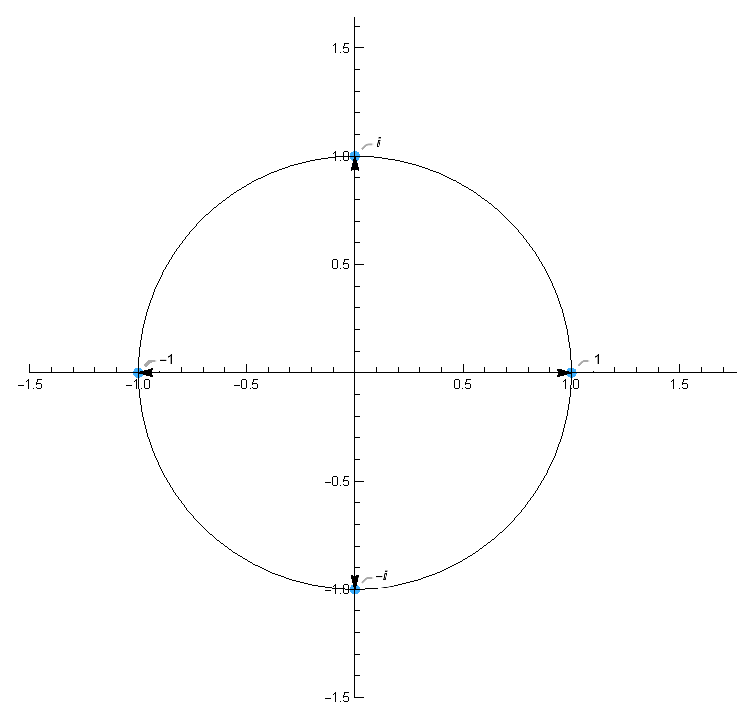
\includegraphics[width = \textwidth]{./figs/chapter_1/Complex_roots_1_n4.eps}
            \caption{$n = 4$}
        \end{subfigure}
    \end{figure}
    \caption{Complex roots of 1 in the plane.}
\end{figure}

In fact, the $n-$th roots of a complex number form a cyclic polygon who's roots lie on a circle centred at the origin with radius $\sqrt[n]{r}.$

\section{Complex Collections}
Regions in the complex plane are of utmost important to the current study. Regions vary both in shape and abstract concepts of inclusion. We shall describe this in detail below. Technically, this section is a special case of applying topology to the complex plane but that is not of too much concern here. To begin with, we shall first define a metric that will be used to study distances in the complex plane.

\begin{defn}[Standard Distance Metric]
    Let $d: \mathbb{C} \times \mathbb{C} \rightarrow \mathbb{R}$ be defined as
    \[
        d(z_1, z_2) := |z - z_{0}| = \sqrt{(z_1 - z_2)^2}.
    \]
    Then, $(\mathbb{C}, d)$ is a metric space.
\end{defn}
It can of course be shown that $d$ is a metric on $\mathbb{C}$ but we consider it to be so for the sake of brevity. The first concept that we must familiarise ourselves with is that of a neighbourhood. In the real numbers a neighbourhood is merely an interval around a given number in the complex plane it is substantially different. 

\begin{defn}[$\epsilon-$Neighbourhood]
    Let $\epsilon > 0$ and $z_{0} \in \mathbb{C}.$ Then, the $\epsilon$ neighbourhood of $z_{0}$ is defined as the set of complex numbers 
    \[
        S(z_0, \epsilon) = \{z \in \mathbb{C}\; |\; d(z, z_0) < \epsilon\}.
    \]
\end{defn}

Given that this is indeed a neighbourhood, we now move on to see what it means for point to lie inside, outside or on the boundary (if it exists) of a such a region.

\begin{defn}[Interior Point]
    Let $z \in X \subseteq \mathbb{C}.$ Then, $z$ is an interior point of $X$ iff
    \[
        \exists\; \epsilon > 0: S(z, \epsilon) \subseteq X.
    \]
\end{defn}

\begin{defn}[Exterior Point]
    Let $z \in X \subseteq \mathbb{C}.$ Then, $z$ is an exterior point of $X$ iff
    $$
        \exists\; \epsilon > 0: S(z, \epsilon) \cap X = \phi.
    $$
\end{defn}	

\begin{defn}[Boundary Point]
    Let $z \in X \subseteq \mathbb{C}.$ Then, $z$ is a boundary point of $X$ iff
    $$
        \exists\; \epsilon > 0\; \land \; z_1 \in X \land z_2 \in \mathbb{C}\backslash X:
            z_1, z_2 \in S(z, \epsilon).
    $$
\end{defn}
Geometrically these definitions only seek to succinctly convey that a point is inside or outside a region. If an $\epsilon-$neighbourhood around that point exists, which lies either completely inside or completely outside the region, respectively. The boundary point defintion captures the fact that a point is on the boundary of a region when an $\epsilon$-neighbourhood contains both points within $X$ and outside $X$. These definitions allow us to simplify the notion of open and closed regions (general concepts from topology) in the context of the complex plane. 

\begin{defn}[Open Set]
    A set $X \subseteq \mathbb{C}$ is open iff
    $$
        \forall\; x \in X: x\;\text{ is an interior point}.
    $$
\end{defn}

\begin{defn}[Closed Set]
    A set $X \subseteq \mathbb{C}$ is closed iff
    $$
        \forall\; x \in X: x\;\text{ is an exterior point}.
    $$
\end{defn}

\begin{defn}[Connected Set]
    A set $X \subseteq \mathbb{C}$ is connected if for each pair of numbers $z_1, z_2 \in X$ there exists a polygonal line contained in $X$ that connects $z_1$ and $z_2$.
    {\color{red} Needs revision and possible breakdown.}
\end{defn}

\begin{defn}[Domain]
    A non-empty set $X \subseteq \mathbb{C}$ which is open and connected. 
\end{defn}

\begin{defn}[Bounded]
    A set $X \subset \mathbb{C}$ is bounded iff
    $$
        \exists\; \epsilon > 0: X \subseteq \{z \in \mathbb{C}\; |\; |z| = \epsilon\}.
    $$
\end{defn}

Connectedness is a much more abstact concept in topology but for the complex plane it is sufficient to view it in the given sense. Boundedness of a set will become increasingly important once we start defining functions on complex sets and see their behaviour.

\begin{exmp}
    $|z - 2 + i| \leq 1.$
\end{exmp}
In the complex plane, the above region looks as follows. It is closed, connected and bounded. Note that it is not a domain. 
\begin{figure}[H]
    \centering
    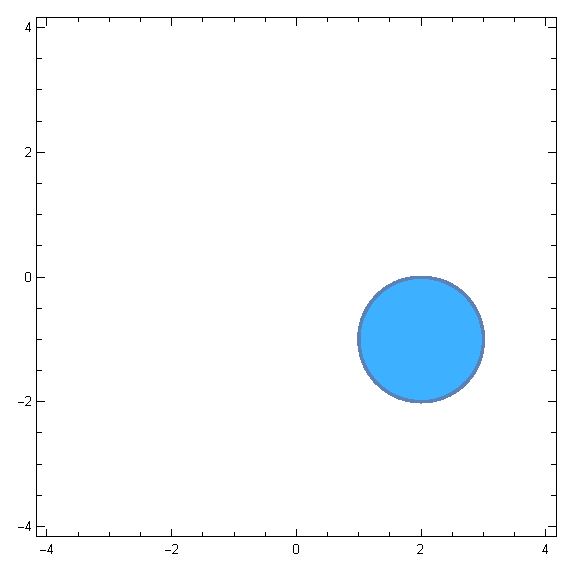
\includegraphics[scale = 0.7]{./figs/chapter_1/region_plot_1.eps}
    \caption{The region $|z - 2 + i| \leq 1$ in blue.}
\end{figure}

\begin{exmp}
    $|2z + 3| \geq 4.$
\end{exmp}
In the complex plane, the above region looks as follows. It is open, connected and unbounded. This region forms a domain.
\begin{figure}[H]
    \centering
    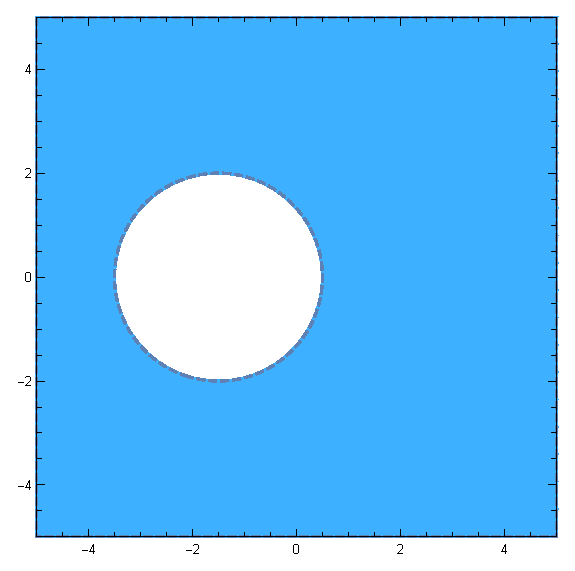
\includegraphics[scale = 0.7]{./figs/chapter_1/region_plot_2.eps}
    \caption{The region $|2z + 3| \geq 4$ in blue.}
\end{figure}


\begin{exmp}
    $0 \leq arg[z] \leq \pi / 4 (z \neq 0).$
\end{exmp}
In the complex plane, the above region looks as follows. It is neither open nor closed, connected and unbounded. This region does not form a domain.
\begin{figure}[H]
    \centering
    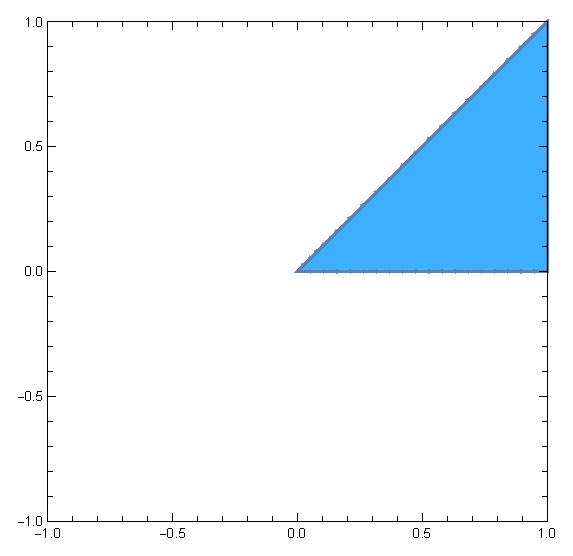
\includegraphics[scale = 0.7]{./figs/chapter_1/region_plot_3.eps}
    \caption{The region $0 \leq arg[z] \leq \pi / 4 (z \neq 0)$ in blue.}
\end{figure}


\begin{exmp}
    $|z - 4| \geq |z|.$
\end{exmp}
In the complex plane, the above region looks as follows. It is closed, connected and unbounded.
\begin{figure}[H]
    \centering
    \includegraphics[scale = 0.7]{./figs/chapter_1/region_plot_4.eps}
    \caption{The region $|z - 4| \geq |z|$ in blue.}
\end{figure}

\chapter{Functions}
\section{Mappings}
In this chapter, we will concern ourselves with mappings of the form $f: X \subseteq \mathbb{C} \rightarrow \mathbb{C}.$ The premise is that such functions can be broken into two parts. One where the real part of the input is mapped to the real part of the output and the other where the imaginary part of the input is mapped to the imaginary part of the output. If we let $z \in X$ and  $w \in \mathbb{C}$ such that $f(z) = w,$ where $z = x + iy$ and $w = u + iv$, then it naturally emerges that

\begin{align*}
    &&f(z) 
        &= w \\
    &\Rightarrow &f(x + iy) 
        &= u + iv \\
\end{align*}

In fact $u$ and $v$ are real valued functions, that in general follow $u, v: \mathbb{R} \times \mathbb{R} \rightarrow \mathbb{R}$ and are parametrised by $x$ and $y$ as $u = u(x, y)$ and $v = v(x, y)$. If we choose to write the complex numbers $z$ and $w$ in polar form, we will get the functions parametrised by the $r$ and $\theta$, the absolute value and the argument. We now take a look at some examples, to observe this complex and real mappings much like how complex numbers are constructed using real numbers. For now, we will take a loot at polynomial-like expressions as we still don't know how complex exponentials or trigonometric functions behave.

\begin{exmp}
    $f(z) = z^2.$
\end{exmp}
We have,
\begin{align*}
    &&f(z) 
        &= z^2 \\
    &\Rightarrow &f(x + iy) 
        &= x^2 - y^2 + 2ixy .
\end{align*}
Therefore, $u(x, y) = x^2 - y^2$ and $v(x, y) = 2xy.$

\begin{exmp}
    $f(z) = |z|^2.$
\end{exmp}
We have,
\begin{align*}
    &&f(z) 
        &= |z|^2 \\
    &\Rightarrow &f(x + iy) 
        &=  x^2 + y^2.
\end{align*}
Therefore, $u(x, y) = x^2 + y^2$ and $v(x, y) = 0.$

\begin{exmp}
    $f(z) = z^3 + z + 1.$
\end{exmp}
We have,
\begin{align*}
    &&f(z) 
        &= z^3 + z + 1\\
    &\Rightarrow &f(x + iy) 
        &= x^3 - 3xy^2 + x + 1 + i(-y^3 + 3x^2y + y).
\end{align*}
Therefore, $u(x, y) = x^3 - 3xy^2 + x + 1$ and $v(x, y) = -y^3 + 3x^2y + y.$

\begin{exmp}
    $f(x + iy) = x^2 - y^2 - 2y + i(2x - 2xy).$
\end{exmp}
We find that $u(x, y) = x^2 - y^2 - 2y$ and $v(x, y) = 2x - 2xy.$
\begin{align*}
    &&f(x + iy) 
        &= x^2 - y^2 - 2y + i(2x - 2xy)\\
    &\Rightarrow &f(x + iy) 
        &= (x - iy)^2 + 2i(x + iy) \\
    &\Rightarrow &f(z)
        &= \overline{z}^{2} + 2iz.
\end{align*}

\begin{exmp}
    $f(z) = z + 1 / z.$
\end{exmp}
We have,
\begin{align*}
    &&f(r, \theta) 
        &= re^{i\theta} + \frac{1}{r}e^{-i\theta}\\
    &\Rightarrow &f(r, \theta)
        &= \left(r + \frac{1}{r}\right)\cos\theta + i\left(r - \frac{1}{r}\right)\sin\theta.
\end{align*}
Therefore, $u(r, \theta) = \left(r + \frac{1}{r}\right)\cos\theta$ and $v(r, \theta) = \left(r - \frac{1}{r}\right)\sin\theta.$

Now, we can extend this notion of writing complex functions in different forms to viewing them as transformations between the planes $xy$ and $uv$. 

\begin{exmp}
    $f(z) = w = z^2.$
\end{exmp}
We have seen that the above function can be broken down into the constituents
$$
    u(x, y) = x^2 - y^2\; \text{and}\; v(x, y) = 2xy,
$$
where $z = x + iy.$ We can now study contours of these functions as they are transformed between the planes $xy$ and $uv$.
\begin{enumerate}
    \item $u = c_1, (c_1 > 0).$
    \begin{enumerate}[label = {(\roman*)}]
        \item 
            $v = 2y\sqrt{y^2 + c_1}, (\infty < y < \infty).$
            \begin{figure}[H]
                \centering
                \begin{subfigure}{0.45\textwidth}
                    \centering
                    \includegraphics[width = \textwidth]{./figs/chapter_1/f_map_1_1.eps}
                    \caption{$xy$-plane}
                \end{subfigure}
                \qquad
                \begin{subfigure}{0.45\textwidth}
                    \centering
                    \includegraphics[width = \textwidth]{./figs/chapter_1/f_map_1_2.eps}
                    \caption{$uv$-plane}
                \end{subfigure}
                \caption{$c_1 = 2.$}
            \end{figure}
        \item 
            $v = -2y\sqrt{y^2 + c_1}, (\infty < y < \infty).$
            \begin{figure}[H]
                \centering
                \begin{subfigure}{0.45\textwidth}
                    \centering
                    \includegraphics[width = \textwidth]{./figs/chapter_1/f_map_2_1.eps}
                    \caption{$xy$-plane}
                \end{subfigure}
                \qquad
                \begin{subfigure}{0.45\textwidth}
                    \centering
                    \includegraphics[width = \textwidth]{./figs/chapter_1/f_map_2_2.eps}
                    \caption{$uv$-plane}
                \end{subfigure}
                \caption{$c_1 = 2.$}
            \end{figure}
    \end{enumerate}
    
    \item $v = c_2, (c_2 > 0).$
    \begin{enumerate}[label = {(\roman*)}]
        \item 
            $u = \frac{c_{2}^{2}}{4y^2} - y^2, (\infty < y < 0).$
            \begin{figure}[H]
                \centering
                \begin{subfigure}{0.45\textwidth}
                    \centering
                    \includegraphics[width = \textwidth]{./figs/chapter_1/f_map_1_3.eps}
                    \caption{$xy$-plane}
                \end{subfigure}
                \qquad
                \begin{subfigure}{0.45\textwidth}
                    \centering
                    \includegraphics[width = \textwidth]{./figs/chapter_1/f_map_1_4.eps}
                    \caption{$uv$-plane}
                \end{subfigure}
                \caption{$c_2 = 2.$}
            \end{figure}
        \item
            $u = x^2 - \frac{c_{2}^{2}}{4x^2}, (0 < x < \infty).$
            \begin{figure}[H]
                \centering
                \begin{subfigure}{0.45\textwidth}
                    \centering
                    \includegraphics[width = \textwidth]{./figs/chapter_1/f_map_2_3.eps}
                    \caption{$xy$-plane}
                \end{subfigure}
                \qquad
                \begin{subfigure}{0.45\textwidth}
                    \centering
                    \includegraphics[width = \textwidth]{./figs/chapter_1/f_map_2_4.eps}
                    \caption{$uv$-plane}
                \end{subfigure}
                \caption{$c_2 = 2.$}
            \end{figure}
    \end{enumerate}
\end{enumerate}

\section{Limiting Processes}
\subsection{Limits}
As in the real numbers it is paramount that we understand limiting processes, to devise methods to study properties of complex mappings. In the plane, the complex limit is similar to that of a two dimensional limit approaching a point.

\begin{defn}[Limit Point]
    Let $x \in X \subseteq \mathbb{C}$, then $x$ is a limit point of $X$ iff
    $$
        \forall \epsilon > 0, \exists y \in X: y \neq x \land y \in S(x, \epsilon).
    $$
\end{defn}
Which is to say a limit point contains points of the concerned set other than itself in every neighbourhood. Limit definitions will now be assumed to be for such limit points. It's interesting to ask what happens when limiting processes are examined relating to points that do not share this property. Well then the definiton for a limit is directly contradicted because it doesn't work for all $\epsilon.$

\begin{defn}[Limit]
    Let $f: X \subseteq \mathbb{C} \rightarrow \mathbb{C},$ then $\lim_{z \rightarrow z_0} f(z) = w (\in \mathbb{C})$ iff $\forall\; \epsilon > 0\; \exists\; \delta(\epsilon) > 0:$
    $$
        0 < d(z, z_0) < \delta(\epsilon) \Rightarrow d(f(z), w) < \epsilon,
    $$ 
    assuming that $z $
\end{defn}
In the following discussion, I will ommit making it explicit that $\delta$ is a function of $\epsilon.$ As for now, it is clear. The above definition can of course delineated as $\lim_{z \rightarrow z_0} f(z) = w (\in \mathbb{C})$ iff $\forall\; \epsilon > 0\; \exists\; \delta > 0:$
$$
    z \in S(z_0, \delta) \Rightarrow f(z) \in S(w, \epsilon).
$$  
This lends to the visualisation.
\begin{figure}[H]
    \centering
    \begin{subfigure}{0.45\textwidth}
        \centering
        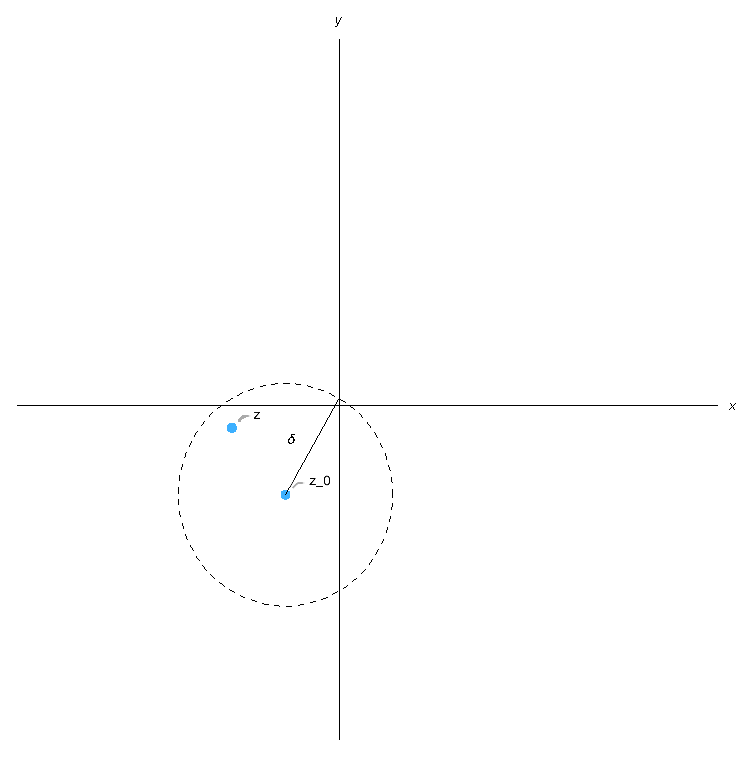
\includegraphics[width = \textwidth]{./figs/chapter_1/limits_def_2.eps}
        \caption{$xy$-plane}
    \end{subfigure}
    \qquad
    \begin{subfigure}{0.45\textwidth}
        \centering
        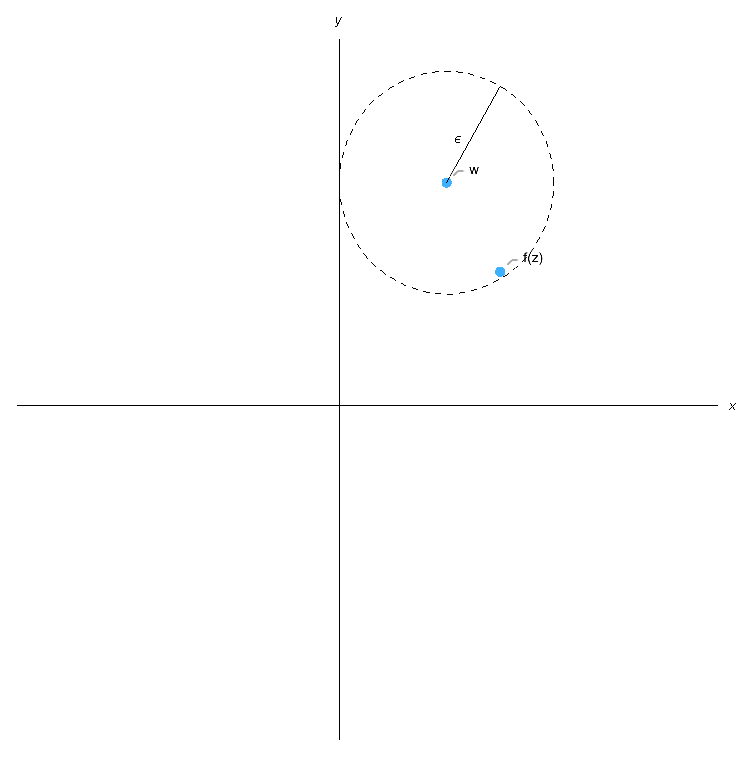
\includegraphics[width = \textwidth]{./figs/chapter_1/limits_def_1.eps}
        \caption{$uv$-plane}
    \end{subfigure}
    \caption{Limits and neighobouehoods.}
\end{figure}

Keeping in line with our previous breakdown of complex functions into constituent parts, we can now use the above definition to define the existence of the complex limit using the real and imaginary function parts. In fact, this will allow us to use other properties of functions by referring to the constituent parts of the complex function.

\begin{thm}[Part Limits]
    Suppose that $f: X \subseteq \mathbb{C} \rightarrow \mathbb{C}$ is a complex function, let $f(z) = u(x, y) + iv(x, y),$ where $z = x + iy$, $z_0 = x_0 + iy_0$, and $w_0 = u_0 + iv_0,$ where $u_0 = u(x_0, y_0)$ and $u_0 = u(x_0, y_0)$. Then, 
    $$
        \lim_{z \rightarrow z_0} f(z) = w_0
    $$ 
    iff 
    $$
        \lim_{(x, y) \rightarrow (x_0, y_0)} u(x, y) = u_0\; \text{and}\; \lim_{(x, y) \rightarrow (x_0, y_0)} v(x, y) = v_0.
    $$
\end{thm}
\begin{proof}
    $\mathbf{[\Rightarrow]}$ Assume that $\lim_{z \rightarrow z_0} f(z) = w_0.$ Then, by definiton, $\forall \epsilon > 0\; \exists\; \delta > 0:$
    $$
       0 < d(z, z_0) < \delta \Rightarrow d(f(z), w_0) < \epsilon.
    $$
    This implies that 
    $$
        \abs{(x - x_0) + i(y - y_0)} < \delta \Rightarrow \abs{(u(x, y) - u_0) + i(v(x, y) - v_0)} < \epsilon.
    $$
    Now, 
    $$
        \abs{Re(u(x, y) - u_0 + i(v(x, y) - v_0))} \leq \abs{u(x, y) - u_0 + i(v(x, y) - v_0))}
    $$
    and 
    $$
        \abs{Im(u(x, y) - u_0 + i(v(x, y) - v_0))} \leq \abs{u(x, y) - u_0 + i(v(x, y) - v_0))}.
    $$
    Whenever $0 < \sqrt{(x - x_0)^2 + (y - y_0)^2} < \delta$, we have
    $$
        \abs{(u(x, y) - u_0)} < \epsilon
    $$
    and 
    $$
        \abs{(v(x, y) - v_0)} < \epsilon.
    $$
    Hence,
    $$
        \lim_{(x, y) \rightarrow (x_0, y_0)} u(x, y) = u_0\; \text{and}\; \lim_{(x, y) \rightarrow (x_0, y_0)} v(x, y) = v_0.
    $$

    $\mathbf{[\Rightarrow]}$ For the converse, assume that $\lim_{(x, y) \rightarrow (x_0, y_0)} u(x, y) = u_0\; \text{and}\; \lim_{(x, y) \rightarrow (x_0, y_0)} v(x, y) = v_0.$ Then, $\forall\; \epsilon > 0$:
    $$
        \exists\; \delta: 0 < \sqrt{(x - x_0)^2 + (y - y_0)^2} < \delta_1 \Rightarrow d(u(x, y), u_0) < \epsilon / 2
    $$
    and
    $$
        \exists\; \delta: 0 < \sqrt{(x - x_0)^2 + (y - y_0)^2} < \delta_2 \Rightarrow d(v(x, y), v_0) < \epsilon / 2.
    $$ 
    If we are to choose, $\delta = \min(\delta_1, \delta_2),$ then 
    \begin{align*}
        \abs{f(z) - w_0}
            &=
                \abs{u + iv - (u_0 + iv_0)} \\
            &= 
                \abs{u - u_0 + i(v - v_0)} \\
            &\leq
                \abs{u - u_0} + \abs{v - v_0} \\
            &\leq
                \epsilon.
    \end{align*}
    Which leads to the conclusion that 
    $$
        \lim_{z \rightarrow z_0} f(z) = w_0
    $$
    This closes the proof.
\end{proof}

\begin{thm}[Uniqueness of Limits]
    If the limit of a function $f: X \subseteq \mathbb{C} \rightarrow \mathbb{C}$ exists at some point $z_0,$ then it is unique.
\end{thm}
\begin{proof}
    We assume that the limit is not unique for the purposes of arriving at a contradiction. Specifically, let 
    $$
        \lim_{z \rightarrow z_0} f(z) = w_1, w_2, (w_1 \neq w_2).
    $$
    Then, by defintion $\forall\; \epsilon > 0$
        $$
            \exists \delta > 0: 0 < d(z, z_0) < \delta \Rightarrow d(f(z), w_1) < \epsilon / 2,
        $$
        $$
            \exists \delta > 0: 0 < d(z, z_0) < \delta \Rightarrow d(f(z), w_2) < \epsilon / 2.
        $$
    Then, by the triangle inequality
        \begin{align*}
            d(w_1, w_2)
                &\leq 
                    d(f(z), w_1) + d(f(z), w_2) \\
                &\leq
                    \epsilon / 2 + \epsilon / 2 \\
                &\leq
                    \epsilon.
        \end{align*}
    Which contradicts the fact that $w1 \neq w_2$ as $w_1$ and $w_2$ cannot be arbitrarily close to each other. This closes the proof.
\end{proof}

\begin{exmp}
    $\lim_{z \rightarrow 1} \frac{i\overline{z}}{3} = \frac{i}{3}, (|z| < 1).$
\end{exmp}
\begin{align*}
    d\left(f(z), \frac{i}{3}\right)
        &=
            d\left(\frac{i\overline{z}}{3}, \frac{i}{3}\right) \\
        &=
            \abs{\frac{i}{3}}d(\overline{z}, 1) \\
        &=
            \frac{1}{3}d(z, 1).
\end{align*}
Therefore, if we choose $\delta(\epsilon) := 3\epsilon$, then the condition $d(z, 1) < \delta$ enforces that $d(f(z), i / 3) < \epsilon.$  

\begin{exmp}
    $\lim_{z \rightarrow 0}\frac{z}{\overline{z}}$ does not exist.
\end{exmp}
We can see this fact by taking the limit approaching from different directions. For the first we set $z = x + i0.$ Then,
\begin{align*}
    \lim_{z \rightarrow x + i0} \frac{z}{\overline{z}}
        &= 
            \lim_{x \rightarrow 0} \frac{x}{x} \\
        &= 
            1.
\end{align*}
We now set $z = 0 + iy.$ Then,
\begin{align*}
    \lim_{z \rightarrow 0 + iy} \frac{z}{\overline{z}}
        &= 
            \lim_{y \rightarrow 0} \frac{y}{-y} \\
        &= 
            -1.
\end{align*}
Which implies that the limit does not exist. As the limit from any given direction of approach must be consistent.

\begin{exmp}
    $$
        \lim_{z \rightarrow z_0} Re(z) = Re(z_0).
    $$
\end{exmp}
\begin{align*}
    d(Re(z), Re(z_0)) 
        &\leq
            d(z, z_0) \\
\end{align*}
Therefore, if we choose $\delta(\epsilon) := \epsilon$, then the condition $d(z, z_0) < \delta$ enforces that $d(Re(z), Re(z_0)) < \epsilon.$  

\begin{exmp}
    $$
        \lim_{z \rightarrow z_0} \overline{z} = \overline{z_0}.
    $$
\end{exmp}
\begin{align*}
    d(\overline{z}, \overline{z_0}) 
        &\leq
            d(z, z_0) \\
\end{align*}
Therefore, if we choose $\delta(\epsilon) := \epsilon$, then the condition $d(z, z_0) < \delta$ enforces that $d(Re(z), Re(z_0)) < \epsilon.$ 

\begin{exmp}
    $$
        \lim_{z \rightarrow z_0} \frac{\overline{z}^{2}}{z} = 0.
    $$
\end{exmp}
\begin{align*}
    d\left(\frac{\overline{z}^{2}}{z}, 0\right) 
        &=
           \abs{\frac{\overline{z}^{2}}{z}} \\
        &= 
            \frac{\abs{\overline{z}^{2}}}{\abs{z}} \\
        &=
            \abs{z}.
\end{align*}
Therefore, if we choose $\delta(\epsilon) := \epsilon$, then the condition $d(z, z_0) < \delta$ enforces that $d\left(\frac{\overline{z}^{2}}{z}, 0\right) < \epsilon.$ 

\begin{exmp}
    $$
        \lim_{z \rightarrow z_0} z^2 + c = z_{0}^{2} + c.
    $$
\end{exmp}
\begin{align*}
    d\left(z^2 + c, z_{0}^{2} + c\right) 
        &=
           d(z^{2}, z_{0}^{2}) \\
        &= 
            \abs{z + z_0}\abs{z - z_0} \\
        &\leq
            (\abs{z} + \abs{z_0})\abs{z - z_0}.
\end{align*}
If we choose $\abs{z - z_0} < 1,$ then
$$
    \abs{z} - \abs{z_0} \leq \abs{\abs{z} - \abs{z_0}} \leq \abs{z - z_0} \leq 1.
$$
We get that, $\abs{z} \leq 1 + \abs{z_0}.$ Finally,
$$
    d\left(z^2 + c, z_{0}^{2} + c\right) \leq (1 +2 \abs{z_0}) \abs{z - z_0}.
$$
Therefore, if we choose $\delta(\epsilon) := \min(1, \epsilon / (1 + 2|z_0|))$, then the condition $d(z, z_0) < \delta$ enforces that $d\left(z^2 + c, z_{0}^{2} + c\right)  < \epsilon.$ 

We finally see the familiar limit properties. 
\begin{thm}[Limit Properties]
    Suppose that $f, g: X \subseteq \mathbb{C} \rightarrow \mathbb{C}$ and $\lim_{z \rightarrow z_0}f(z) = w_1,$ $\lim_{z \rightarrow z_0}g(z) = w_2,$ where $w_1, w_2 \in \mathbb{C}$ and $w_1, w_2 < \infty.$ Then,
    \begin{enumerate}[label = {(\roman*)}] 
        \item
            $$
                \lim_{z \rightarrow z_0} (f(z) \pm g(z)) = w_1 \pm w_2,
            $$
        \item
            $$
                \lim_{z \rightarrow z_0} (f(z)g(z)) = w_1w_2,
            $$
        \item
            $$
                \lim_{z \rightarrow z_0} (f(z) / g(z)) = w_1 / w_2,
            $$
            provided that $w_2 \neq 0.$
    \end{enumerate}
\end{thm}

\subsubsection{Stereographic Projection}
To provide definitions for infinite limits or limits at infinity, we must do a bit more work. As in the real case, it is not straightforward to define such limits. This arises due to the fact that that limiting processes in the plane have an infinte number of directions from which they can act. To circumvent this problem, we project the complex plane onto a sphere. From each point on the pane we may draw a line to the north pole (N) (point $(0, 0, 1)$ of the unit sphere. The resulting intersection of that line with the sphere creates a point on the sphere (P) which is the required projection. The north pole is called the point at \textit{infinity}. Points exterior to the unit sphere correspond to projections on the upper hemisphere, while points interior to the unit sphere correspond to projections on the lower hemisphere.

\begin{figure}[H]
    \centering
    \includegraphics[trim = 20 0 0 0, scale = 0.7, clip]{./figs/chapter_1/stereo_projection.eps}
    \caption{Stereographic Projection}
\end{figure}

For $\epsilon > 0$ points outside $\abs{z} = 1 / \epsilon$ are members of an $\epsilon-$neighbourhood of infinity (North Pole). Armed with this construct we can now define other familiar limits in the complex plane. Since they are defined using previous definitions of the limit, they are stated as a theorem.

\begin{thm}[Unsual Limits]
    If $f: X \subseteq \mathbb{C} \rightarrow \mathbb{C}$ and $z_0 \in X, w_0 \in \mathbb{C}$, then 
    \begin{enumerate}[label = {(\roman*)}]
        \item
            $$
                \lim_{z \rightarrow z_0} f(z) = \infty \iff \lim_{z \rightarrow z_0} \frac{1}{f(z)} = 0,
            $$
        \item
            $$
                \lim_{z \rightarrow \infty} f(z) = w_0 \iff \lim_{z \rightarrow 0} f\left(\frac{1}{z}\right) = w_0,
            $$
        \item
            $$
                \lim_{z \rightarrow \infty} f(z) = \infty \iff \lim_{z \rightarrow 0} \frac{1}{f(1/z)} = 0.
            $$
    \end{enumerate}
\end{thm}

\begin{proof}
    \begin{enumerate}[label = {(\roman*)}]
        \item
            $\mathbf{[\Rightarrow]}$ Assume that $\lim_{z \rightarrow z_0} f(z) = \infty.$ Then,
            $$
                \forall\; \epsilon > 0\; \exists\; \delta > 0: \; 0 < d(z, z_0) < \delta \Rightarrow \abs{f(z)} > \frac{1}{\epsilon}.
            $$
            In other words, $f(z)$ is in the $\epsilon-$neighobouhood of infinity. This means that 
            \begin{align*}
                &&\abs{f(z)} 
                    &> 
                        \frac{1}{\epsilon} \\
                &\Rightarrow &\frac{1}{\abs{f(z)}}
                    &<
                        \epsilon \\
                &\Rightarrow &\abs{\frac{1}{f(z)} - 0}
                    &<
                        \epsilon.
            \end{align*}
            $\mathbf{[\Rightarrow]}$ Conversely, let $\lim_{z \rightarrow z_0} \frac{1}{f(z)} = 0.$ Then,
            $$
                \forall\; \epsilon > 0\; \exists\; \delta > 0: \; 0 < d(z, z_0) < \delta \Rightarrow \abs{\frac{1}{f(z)}} < \epsilon.
            $$
            \begin{align*}
                &&\abs{\frac{1}{f(z)}}
                    &< 
                        \epsilon \\
                &\Rightarrow &\abs{f(z)}
                    &>
                        \frac{1}{\epsilon}.
            \end{align*}
        \item
            $\mathbf{[\Rightarrow]}$ Assume that $\lim_{z \rightarrow \infty} f(z) = w_0.$ Then,
            $$
                \forall\; \epsilon > 0\; \exists\; \delta > 0: \; \abs{z} > \frac{1}{\delta} \Rightarrow d(f(z), w_0) < \epsilon.
            $$
            This can be written as
            $$
                \forall\; \epsilon > 0\; \exists\; \delta > 0: \; \frac{1}{\abs{z}} < \delta \Rightarrow d(f(1/z), w_0) < \epsilon.
            $$
            $\mathbf{[\Rightarrow]}$ Conversely, suppose that $\lim_{z \rightarrow 0} f\left(\frac{1}{z}\right) = w_0.$ Then, 
            $$
                \forall\; \epsilon > 0\; \exists\; \delta > 0: \; \frac{1}{\abs{z}} < \delta \Rightarrow d(f(1/z), w_0) < \epsilon,
            $$
            which can be written as
            $$
                \forall\; \epsilon > 0\; \exists\; \delta > 0: \; \abs{z} > \frac{1}{\delta} \Rightarrow d(f(z), w_0) < \epsilon.
            $$
        \item
            $\mathbf{[\Rightarrow]}$ Assume that $\lim_{z \rightarrow \infty} f(z) = \infty.$ Then,
            $$
                \forall\; \epsilon > 0\; \exists\; \delta > 0: \; \abs{z} > \frac{1}{\delta} \Rightarrow \abs{f(z)} > \frac{1}{\epsilon}.
            $$
            This implies
            \begin{align*}
                &&\forall\; \epsilon > 0\; \exists\; \delta > 0: 
                    &\abs{z} > \frac{1}{\delta} \Rightarrow \abs{f(z)} > \frac{1}{\epsilon} \\
                &\Rightarrow &\forall\; \epsilon > 0\; \exists\; \delta > 0:
                    &0 < \frac{1}{\abs{z}} < 1 / \delta \Rightarrow \frac{1}{\abs{f(1/z)}} < \epsilon \\
                &\Rightarrow &\forall\; \epsilon > 0\; \exists\; \delta > 0:
                    &0 < \abs{z} < \delta \Rightarrow \frac{1}{\abs{f(1/z)}} < \epsilon.  
            \end{align*}
            $\mathbf{[\Rightarrow]}$ Conversely, we assume $\lim_{z \rightarrow 0} \frac{1}{f(1/z)} = 0.$ Then, 
            $$
                \forall\; \epsilon > 0\; \exists\; \delta > 0: 0 < \abs{z} < \delta \Rightarrow \frac{1}{\abs{f(1/z)}} < \epsilon.
            $$
            We may conclude that 
            $$
                \forall\; \epsilon > 0\; \exists\; \delta > 0: \abs{z} > \frac{1}{\delta} \Rightarrow \abs{f(z)} > \frac{1}{\epsilon}.
            $$
    \end{enumerate}
    This closes the proof.
\end{proof}


\begin{exmp}
    $$
        \lim_{z \rightarrow -1} \frac{z + 1}{iz + 3} = 0.
    $$
\end{exmp}
\begin{align*}
    &&\lim_{z \rightarrow -1} \frac{z + 1}{iz + 3} 
        &= 
            0 \\
    &\iff &\lim_{z \rightarrow -1} \frac{iz + 3}{z + 1} 
        &= 
            \infty.
\end{align*}

\begin{exmp}
    $$
        \lim_{z \rightarrow \infty} \frac{2z^3 - 1}{z^2 + 1} = \infty.
    $$
\end{exmp}
\begin{align*}
    &&\lim_{z \rightarrow \infty} \frac{2z^3 - 1}{z^2 + 1} 
        &= 
            \infty \\
    &\iff &\lim_{z \rightarrow 0} \frac{(1/z^2) + 1}{2(1/z^3) - 1} 
        &= 
            0 \\
    &\iff &\lim_{z \rightarrow 0} z\frac{1 + z^2}{2 - z^3}  
        &= 
            0.
\end{align*}

\subsection{Continuity}
\begin{defn}[Continuous Functions]
    A function $f: X \subseteq \mathbb{C} \rightarrow \mathbb{C}$, is continuous at a point $z_0 \in X$ iff
    $$
        \forall\; \epsilon\; \exists\; \delta >: 0 < d(z, z_0) < \delta(\epsilon) \Rightarrow d(f(z), f(z_0)) < \epsilon,
    $$
    which is to say that
    $$
        \lim_{z \rightarrow z_0} f(z) = f(z_0).
    $$
\end{defn}

\begin{thm}[Continuous Composition]
    Let $f: X \subseteq \mathbb{C} \rightarrow dom(g) \subseteq \mathbb{C}$ and $g: Y \subseteq rng(f) \rightarrow \mathbb{C}$ such that $f$ is continous at some point $z_0 \in X$ and $g$ is continuous at $f(z_0) \in Y.$ 
\end{thm}
\begin{proof}
    By defintion, 
    $$
        \forall\; \epsilon > 0\; \exists\; \delta_1 > 0: 0 < d(f(z), f(z_0)) < \delta_1 \Rightarrow d(g(f(z)), g(f(z_0))) < \epsilon,
    $$
    where $f(z) \in Y.$ Then, 
    \begin{align*}
        &&\text{For}\; \delta_1 > 0\; \exists \delta_2 > 0: 
            &0 < d(z, z_0) < \delta_2 \Rightarrow d(f(z), f(z_0)) < \delta_1, \\
        &\Rightarrow &\text{For}\; \delta_1 > 0\; \exists \delta_2 > 0: 
            &0 < d(z, z_0) < \delta_2 \Rightarrow d(g(f(z)), g(f(z_0))) < \epsilon.
    \end{align*}
\end{proof}

\begin{thm}[Non Vanishing Continuity]
    If a function $f: X \subseteq \mathbb{C} \rightarrow \mathbb{C}$ is continuous and non-zero at a point $z_0 \in X$, then 
    $$
        \exists\; \epsilon > 0: \; f(z') \neq 0\; \forall z' \in S(z_0, \epsilon).
    $$ 
\end{thm}
\begin{proof}
From the definiton of continuity, for $\epsilon = \abs{f(z_0) / 2},$
    $$
        \exists\; \delta > 0: \; d(f(z), f(z_0)) < \abs{\frac{f(z_0)}{2}}.
    $$
Now, if we assume that $\exists\; z' \in S(z_0,\delta): f(z') = 0$, we would get
    \begin{align*}
        &&\abs{z} - \abs{z_0} \leq \abs{z - z_0} 
            &\leq 
                \abs{\frac{f(z_0)}{2}} \\
        &\Rightarrow &\abs{f(z_0)}
            &\leq
                \abs{\frac{f(z_0)}{2}}.
    \end{align*}
This is a clear contradiction.
\end{proof}

\begin{thm}[Boundedness]
    If a function $f: X \subseteq \mathbb{C} \rightarrow \mathbb{C}$ is continuous on the closed and bounded region $R \subseteq X,$ then 
    $$
        \exists\; \epsilon > 0: \; \abs{f(z)} \leq \epsilon, z \in R.
    $$
    That is to say, that $f$ is bounded in the region. Equality will hold for a particular $z \in R.$
\end{thm}
\begin{proof}
    Let $f(z) = u(x, y) + iv(x, y),$ where $u, v: \mathbb{R}^{2} \rightarrow \mathbb{R}.$ Since $f$ is continuous on $R$ so are $u$ and $v.$ Since $R$ is closed and boundeded, $\exists z' = x' + iy', z'' = x'' + iy'' \in R: $
    $$
        \sup_{(x, y) \in R} u(x, y) = \max_{(x, y) \in R} u(x, y) = u(x', y')
    $$
    and
    $$
        \sup_{(x, y) \in R} v(x, y) = \max_{(x, y) \in R} v(x, y) = v(x'', y'')
    $$
    This allows us to constrain $f$ in $R$ as follows:
    $$
        \abs{f(z)} \leq \sqrt{u(x', y')^2 + v(x'', y'')^2}.
    $$
This concludes the proof.
\end{proof}

\begin{thm}[Vanishing Limits]
    Let $f: X \subseteq \mathbb{C} \rightarrow \mathbb{C}$ and $g: Y \subseteq \mathbb{C} \rightarrow \mathbb{C}$ such that $\lim_{z \rightarrow z_0}f(z) = 0.$ If $g(z) \leq M$ in some neighbourhood of $z_0$, then
    $$
        \lim_{z \rightarrow z_0}f(z)g(z) = 0.
    $$
\end{thm}
\begin{proof}
    By definition, 
    $$
        \forall\; \epsilon > 0\; \exists\; \delta > 0: 0 < d(z, z_0) < \delta \Rightarrow \abs{f(z)} < \epsilon.
    $$
    Now, if $\exists\; \delta_1 > 0: \abs{g(z)} < M$ in $S(z_0, \delta_1).$ Then, choosing $\gamma = \min(\delta, \delta_1)$ gives us
    $$
        0 < d(z, z_0) < \gamma \Rightarrow \abs{f(z)g(z)} < \epsilon.
    $$   
\end{proof}

\subsection{Derivatives}
Derviatives of complex functions are defined similarly to derivatives of real functions. In fact, as we have seen so far, we can relate limiting processes to the real constiuent functions of the complex function, we can do the same for derivatives. This theorem would be quite useful in the future. For now, we start with a formal definiton.

\begin{defn}[Derivative]
    Let $f: X \subseteq \mathbb{C} \rightarrow \mathbb{C}$ be a complex function and let $f$ be defined in some $\epsilon-$neighbourhood of $z_0$. Then,
    $$
        f'(z_0) := \lim_{z \rightarrow z_0} \frac{f(z) - f(z_0)}{z - z_0}.
    $$
    Provided, the limit exists.
\end{defn}
For a more familiar version of the above defintion we may define the following quantities.
$$
    \Delta z: = z - z_0, d(z, z_0) < \epsilon
$$
where $\epsilon > 0$ is an in the above definition and 
$$
    \Delta w := f(z_0 + \Delta z) - f(z_0).
$$ 
Then,
$$
    f'(z_0) := \left.\frac{df}{dz}\right|_{z = z_0} := \lim_{\Delta z \rightarrow 0} \frac{\Delta w}{\Delta z}.
$$

\begin{exmp}
    $$
        f(z) = z^2, z \in \mathbb{C}.
    $$
\end{exmp}
\begin{align*}
    f'(z)
        &= 
            \lim_{\Delta z \rightarrow 0} \frac{\Delta w}{\Delta z} \\
        &= 
            \lim_{\Delta z \rightarrow 0} \frac{(z + \Delta z)^2 - z^2}{\Delta z} \\
        &=
            \lim_{\Delta z \rightarrow 0} \Delta z + 2z \\
        &=
            2z.
\end{align*}

\begin{exmp}
    $$
        f(z) = \overline{z}, z \in \mathbb{C}.
    $$
\end{exmp}
\begin{align*}
    f'(z)
        &=
            \lim_{\Delta z \rightarrow 0} \frac{\overline{(z + \Delta z)} - \overline{z}}{\Delta z} \\
        &=
            \lim_{\Delta z \rightarrow 0} \frac{\overline{\Delta z}}{\Delta z}.
\end{align*}
We can see that on the path $(\Delta x, 0),$ the limit is $1$ and on the path $(0, \Delta y),$ the limit is $-1$. This shows that the limit does not exist, which means that the derivative does not exist anywhere in $\mathbb{C}.$

\begin{exmp}
    $$
        f(z) = \abs{z}^2, z \in \mathbb{C}.
    $$
\end{exmp}
\begin{align*}
    \lim_{\Delta z \rightarrow 0} \frac{\Delta w}{\Delta z}
        &= 
            \lim_{\Delta z \rightarrow 0} \frac{\abs{z + \Delta z}^{2} - \abs{z}^2}{\Delta z} \\
        &=
            \lim_{\Delta z \rightarrow 0} \frac{(z + \Delta z)(\overline{z} - \overline{\Delta z}) - \abs{z}^{2}}{\Delta z} \\
        &=
            \lim_{\Delta z \rightarrow 0} \frac{z\overline{\Delta z} + \Delta z \overline{z} + \abs{\Delta z}^{2}}{\Delta z} \\
        &=
            \lim_{\Delta z \rightarrow 0} \left(\overline{z} + \overline{\Delta z}  + z \frac{\overline{\Delta z}}{\Delta z}\right)
\end{align*}
On $(\Delta x, 0)$, we have 
\begin{align*}
    \lim_{\Delta z \rightarrow 0} \frac{\Delta w}{\Delta z}
        &= 
            z + \overline{z}.
\end{align*}
On $(0, \Delta y)$, we have 
\begin{align*}
    \lim_{\Delta z \rightarrow 0} \frac{\Delta w}{\Delta z}
        &= 
            z - \overline{z}.
\end{align*}
By the fact that limits should be unique, we have 
\begin{align*}
    &&z + \overline{z} 
        &= 
            z - \overline{z} \\
    &\Rightarrow &z
        &= 0.
\end{align*}
Therefore, $f'(z)$ exists only when $z = 0.$

\begin{thm}[Chain Rule]
    Suppose that $f: X \subseteq \mathbb{C} \rightarrow \mathbb{C}$ has a derivative at $z_0 \in X$ and $g: Y \subseteq rng(f) \rightarrow \mathbb{C}$ has a derivative at $f(z_0) \in Y$. Then, $g(f(z))$ has a derivative at $z_0$ and 
    $$
        g(f(z_0))' = g'(f(z_0)) f'(z_0).
    $$
\end{thm}
\begin{proof}
    Let $w_0 = f(z_0)$ and $g'(f(z_0)) = g'(w_0).$ Then, $\exists\; \epsilon > 0: g'(w_0) \in S(w_0, \epsilon).$ Define the function
    $$
        \phi(w) = 
            \left\{
                \begin{array}{cc}
                    0 & w = w_0, \\
                    \frac{g(w) - g(w_0)}{w - w_0} & w \neq w_0. \\
                \end{array}
            \right.
    $$
    Now, 
    $$
        \lim_{w \rightarrow w_0} \phi(w) = \lim_{w \rightarrow w_0} \frac{g(w) - g(w_0)}{w - w_0} = g'(w_0).
    $$
    If $f(z)$ is chose to be in $S(w, \epsilon)$, then
    $$
        \frac{g(f(z)) - g(f(z_0))}{f(z) - f(z_0)} = [g'(f(z_0)) + \phi(f(z))]\frac{f(z) - f(z_0)}{z - z_0}.
    $$
    If $z \rightarrow z_0,$ then
    $$
        (g(f(z_0)))' = g'(f(z_0))f'(z_0).
    $$
\end{proof}
We have now reached the point where we can correlate derivatives in the complex plane to multidimensional derivatives in the real plane. This leads us to the \textit{Cauchy-Riemann Equations}.

\begin{thm}[Cauchy-Riemann Equations]
    Suppose that $f: X \subseteq \mathbb{C} \rightarrow \mathbb{C}$ can be written as 
    $$
        f(z) := u(x, y) + iv(x, y),
    $$
    where $u(x, y), v(x, y): \mathbb{R}^{2} \rightarrow \mathbb{R}.$ Further, assume that $f'(z_0)$ exists for some $z_0 = x_0 + iy_0 \in X.$ Then, 
    $$
        \frac{\partial u(x, y)}{\partial x}, \frac{\partial u(x, y)}{\partial y}, \frac{\partial v(x, y)}{\partial x}\; \text{and}\; \frac{\partial v(x, y)}{\partial y}\; \text{exist}
    $$
    and 
    $$
        \frac{\partial u(x_0, y_0)}{\partial x} = \frac{\partial v(x_0, y_0)}{\partial y},
    $$
    $$
        \frac{\partial u(x_0, y_0)}{\partial y} = -\frac{\partial v(x_0, y_0)}{\partial x}.
    $$
    Finally, 
    $$
        f'(z_0) = \frac{\partial u(x_0, y_0)}{\partial x} + i\frac{\partial v(x_0, y_0)}{\partial x}.
    $$
\end{thm}
\begin{proof}
    Since $f'(z_0)$ exists, we have from our limit defintions that
    $$
        f'(z_0) = \lim_{(\Delta x, \Delta y) \rightarrow (0, 0)} Re\left(\frac{\Delta w}{\Delta z}\right) + \lim_{(\Delta x, \Delta y) \rightarrow (0, 0)} Im\left(\frac{\Delta w}{\Delta z}\right),
    $$
    where 
    \begin{align*}
        \frac{\Delta w}{\Delta z}
            &=
                \frac{f(z + z_0) - f(z_0)}{\Delta z} \\
            &=
                \frac{u(x_0 + \Delta x, y_0 + \Delta y) - u(x_0, y_0)}{\Delta x} + i\frac{v(x_0 + \Delta x, y_0 + \Delta y) - v(x_0, y_0)}{\Delta y}.
    \end{align*} 
    Since we know that the limit exists and must be unique, the limit on the paths $(0, \Delta y)$ and $(\Delta x, 0)$ should be equal. We must have

    \noindent $(\Delta x, 0):$
    \begin{align*}
        \lim_{(\Delta x, \Delta y) \rightarrow (0, 0)} Re\left(\frac{\Delta w}{\Delta z}\right)
            &= 
                \lim_{\Delta x \rightarrow 0} \frac{u(x_0 + \Delta x, y_0) - u(x_0, y_0)}{\Delta x} \\
            &=
                \frac{\partial u(x_0, y_0)}{\partial x} \\
    \end{align*}
    \begin{align*}
        \lim_{(\Delta x, \Delta y) \rightarrow (0, 0)} Im\left(\frac{\Delta w}{\Delta z}\right)
            &= 
                \lim_{\Delta x \rightarrow 0} \frac{v(x_0 + \Delta x, y_0) - v(x_0, y_0)}{\Delta y} \\
            &=
            \frac{\partial v(x_0, y_0)}{\partial x} \\
    \end{align*}

    \noindent $(0, \Delta y):$
    \begin{align*}
        \lim_{(\Delta x, \Delta y) \rightarrow (0, 0)} Re\left(\frac{\Delta w}{\Delta z}\right)
            &= 
                \lim_{\Delta y \rightarrow 0} \frac{v(x_0, y_0 + \Delta y) - v(x_0, y_0)}{\Delta y} \\
            &=
                \frac{\partial v(x_0, y_0)}{\partial y} \\
    \end{align*}
    \begin{align*}
        \lim_{(\Delta x, \Delta y) \rightarrow (0, 0)} Re\left(\frac{\Delta w}{\Delta z}\right)
            &= 
                \lim_{\Delta y \rightarrow 0} \frac{u(x_0, y_0 + \Delta y) - u(x_0, y_0)}{i\Delta y} \\
            &=
                -\frac{\partial u(x_0, y_0)}{\partial y} \\
    \end{align*}
    This provides an expression for $f'(z_0)$ as 
    $$
        f'(z_0) = \frac{\partial u(x_0, y_0)}{\partial x} + i \frac{\partial v(x_0, y_0)}{\partial x} = \frac{\partial v(x_0, y_0)}{\partial y} - i \frac{\partial u(x_0, y_0)}{\partial y}. 
    $$
\end{proof}
The Cauchy-Riemann equations are important as they provide us with necessary conditions for the existence of a derivative of a function in the complex plane. If we would like to discuss the converse, we need to impose stronger conditions on the partial derivatives of $u$ and $v$. This will allow us to write the following.
\begin{thm}[Derivative Existence]
    Suppose that $f: X \subseteq \mathbb{C} \rightarrow \mathbb{C}$ can be written as 
    $$
        f(z) := u(x, y) + iv(x, y),
    $$
    If $u$ and $v$ have continuous partial derivatives on $X$ and satisfy the Cauchy-Riemann equations, then $f$ is differentiable on $X$.
\end{thm}

\begin{exmp}
    $f(z) = z^2.$ 
\end{exmp}
We have seen that $f$ is differentiable in $\mathbb{C}$ in \exmpref{2.2.9}. We may now see that the components of $f$ satisfy the Cauchy-Riemann equations. It is clear that
\[
    f(x + iy) = x^2 - y^2 + 2ixy.
\]
From this, we can see that $u(x, y) = x^2 - y^2$ and $v(x, y) = 2xy$. We have,
\[
    \begin{array}{cc}
        \frac{\partial u(x, y)}{\partial x} = 2x & \frac{\partial u(x, y)}{\partial y} = -2y \\
        \frac{\partial v(x, y)}{\partial x} = 2y & \frac{\partial v(x, y)}{\partial y} = 2x.
    \end{array}
\]
Which satisfy the Cauchy-Riemann equations.

\begin{exmp}
    $f(z) = |z|^2.$
\end{exmp}
As seen in \exmpref{2.2.11}, $f$ is only differentiable at $z = 0.$ We can breakdown $f$ into 
\[
    f(x + iy) = x^2 + y^2,
\]
which means that $u(x, y) = x^2 + y^2$ and $v(x, y) = 0.$ Then,
\[
    \begin{array}{cc}
        \frac{\partial u(x, y)}{\partial x} = 2x & \frac{\partial u(x, y)}{\partial y} = 2y \\
        \frac{\partial v(x, y)}{\partial x} = 0 & \frac{\partial v(x, y)}{\partial y} = 0.
    \end{array}
\]
These clearly do not satisfy the Cauchy-Riemann equations. 

We now turn to inreasing the strength of our definition of differentiability. It is of much use that a function may be differentiable in an entire region. We give this a special name, an analytic function. Although we will define it more precisely, the idea that a function can be differentiable throughout a region is a useful foundation for the extension of functions, which we will encounter later.

\begin{defn}[Analytic Functions]
    A function $f: X \subseteq \mathbb{C} \rightarrow \mathbb{C}$ is analytic at $z_0 \in X$ iff
    \[
        \exists\; \epsilon > 0: f\; \text{is differentiable in}\; S(z_0, \epsilon).
    \] 
    If a function is analytic in $\mathbb{C},$ then $f$ is entire.
\end{defn}

An immediate consequence of this defintion is the well known fact that if a function's derivative is 0 in a region, the function itself must be constant there.
\begin{thm}[Vanishing Derivative]
    Suppose that $f: X \subseteq \mathbb{C} \rightarrow \mathbb{C}$ and $f'(z) = 0$ in some domain $D \subseteq X.$ Then, 
    $f$ is constant in $D.$
\end{thm}
\begin{proof}
    Let $f(z) = u(x, y) + iv(x, y).$ Then, because $f'(z) = 0$ in $D$, we must have that 
    \begin{align*}
        \frac{\partial u(x, y)}{\partial x} &= \frac{\partial v(x, y)}{\partial y} = 0 \\
        \frac{\partial v(x, y)}{\partial y} &= -\frac{\partial u(x, y)}{\partial x} = 0.
    \end{align*}
    If we let $L$ be a line segment from point $P$ to $P'$ in $D.$ Then,
    \[
        \frac{du}{d\mathbf{s}} = \nabla u \cdot \hat{n} = 0.
    \]
    where $\mathbf{s}$ is the distance vector from $P$ to $P'$ and $\hat{n}$ is the unit vector along $L$ in the direction of increasing $\mathbf{s}$.
    This gives us that 
    \[
        u(x, y) = C\; (\text{constant on}\; L).
    \]
    Since our choice for $L$ was arbitrary, this argument holds for all lines in $D$ and we may conclude that 
    \[
        u(x, y) = C\; (\text{constant in}\; D).
    \]
    The same argument holds for $v(x, y)$ and this closes the proof.
\end{proof}

\begin{exmp}
    $f(z) = \frac{z^3 + 4}{(z^3 - 3)(z^2 + 1)}.$  
\end{exmp}
$f$ is analytic in $\mathbb{C} \backslash \{\pm\sqrt{3}, \pm i\}.$


\begin{exmp}
    $f(z) = \cosh\,x\cos\,y + i \sinh\,x\sin\,y.$  
\end{exmp}
$f$ is analytic in $\mathbb{C},$ i.e. \textit{entire}.

\begin{thm}
    Suppose that $f: X \subseteq \mathbb{C} \rightarrow \mathbb{C}$ and $\overline{f}$ are analytic in a domain $D \subset \mathbb{C}.$ Then, $f$ is constant in $D.$
\end{thm}
\begin{proof}
    Let $f(z) = u_1(x, y) + iv_1(x, y)$ and $\overline{f}(z) = u_2(x, y) + iv_2(x, y).$  Then,
    \begin{align*}
        \frac{\partial u_1(x, y)}{\partial x} &= \frac{\partial v_1(x, y)}{\partial y}, \\
        \frac{\partial u_1(x, y)}{\partial y} &= -\frac{\partial v_1(x, y)}{\partial x}.
    \end{align*}
    and
    \begin{align*}
        \frac{\partial u_2(x, y)}{\partial x} &= \frac{\partial v_2(x, y)}{\partial y}, \\
        \frac{\partial u_2(x, y)}{\partial y} &= -\frac{\partial v_2(x, y)}{\partial x}.
    \end{align*}
    But $u_1(x, y) = u_2(x, y)$ and $v_1(x, y) = - v_2(x, y).$ Therefore,
    \begin{align*}
        &&\frac{\partial u_1(x, y)}{\partial x} 
            &= 
                \frac{\partial v_2(x, y)}{\partial y} \\
        &\Rightarrow &\frac{\partial u_1(x, y)}{\partial x}
            &=
                0 \\
        &\Rightarrow &\frac{\partial v_1(x, y)}{\partial x}
            &=
                0.
    \end{align*}
    Hence, $f$ is constant in $D$.
\end{proof}

\begin{thm}
    If a function $f: X \subseteq \mathbb{C} \rightarrow \mathbb{C}$ is analytic in a domain $D \subset \mathbb{C},$ where $\abs{f(z)}$ is constant, then $f$ is constant in $D.$
\end{thm}
\begin{proof}
    We have that
    \[
        \abs{f(z)} = C\; (\text{constant in}\; D).
    \]
    Clearly, if $C = 0$, then $f$ vanishes throughout $D$. If $C \neq = 0$, then
    \begin{align*}
        &&f(z)\overline{f(z)} 
            &= 
                C^2, \forall\; z \in D \\
        &\Rightarrow &\overline{f(z)} 
            &=
                \frac{C^2}{f(z)}, \forall\; z \in D \\
        &\Rightarrow &\overline{f(z)}\;
            &\text{is analytic in D.}
    \end{align*}
    Hence, $f$ is constant in $D$.
\end{proof}

\begin{exmp}
    $f(x, y) = 3x + y + i(3y - x), x, y \in \mathbb{R}^{2}.$
\end{exmp}
We have that $u(x, y) = 3x + y$ and $v(x, y) = 3y - x.$ The partial deriatives are
\[
    \begin{array}{cc}
        \frac{\partial u(x, y)}{\partial x} = 3 & \frac{\partial u(x, y)}{\partial y} = 1 \\
        \frac{\partial v(x, y)}{\partial x} = -1 & \frac{\partial v(x, y)}{\partial y} = 3 \\
    \end{array}
\]
The first order partial derivatices of $u$ and $v$ are continuous in $\mathbb{R}^{2}$ and satisfy the Cauchy-Riemann equations. This means that $f$ is analytic in $\mathbb{C}.$

\begin{exmp}
    $f(z) = (z^2 - 2)e^{-z}.$
\end{exmp}
\begin{align*}
    f(x, y)
        &=
            (x^2 - 2)e^{-x - iy} + 2ixye^{-x - iy} - 2e^{-x - iy} \\
        &=
            [(x^2 - y^2 -2)\cos y + 2xy\sin y]e^{-x} + i[-(x^2 - y^2)\sin y + 2xy\cos y + 2\sin y]e^{-x}.
\end{align*} 
Therefore,
\[
    u(x, y) = [(x^2 - y^2 -2)\cos y + 2xy\sin y]e^{-x} 
\]
and
\[
    v(x, y) = [-(x^2 - y^2)\sin y + 2xy\cos y + 2\sin y]e^{-x}.
\]
We have,
\begin{equation*}
    \begin{split}
        \frac{\partial u(x, y)}{\partial x} 
            &= 
                (-e^{-x})[(2 x \cos y + 2 y \sin y)\left(\left(x^2 - y^2 - 2\right) \cos y + 2 x y\sin y \right) \\
            &- 
                \left(\left(x^2 - y^2 - 2\right) \cos y + 2xy\sin y\right)].
    \end{split}
\end{equation*}
\begin{equation*}
    \begin{split}
        \frac{\partial u(x, y)}{\partial y} 
            &= 
            (-e^{-x})[( -\left( x^2 - y^2 - 2 \right) \sin y + 2x\sin y + 2xy\cos y - 2y \cos y )\\
            &
                e^{-x}\left( \left(x^2 - y^2 - 2 \right) \cos y + 2xy\sin y \right)].
    \end{split}
\end{equation*}
\begin{equation*}
    \begin{split}
        \frac{\partial v(x, y)}{\partial x}
            &= 
                (-e^{-x}) [(2y\cos y - 2x\sin y)((y^2 - x^2)\sin y + 2xy \cos y + 2\sin y) \\
            &+ 
                ((y^2 - x^2)\sin y + 2xy\cos y + 2 \sin y].
    \end{split}
\end{equation*}
\begin{equation*}
    \begin{split}
        \frac{\partial v(x, y)}{\partial y}
           &= 
                (-e^{-x}) [(y^2 - x^2) \cos y - 2xy\sin y + 2x\cos y + 2y\sin y + 2\cos y] \\
            &
                [(y^2 - x^2)\sin y + 2xy\cos y + 2\sin y]
    \end{split}
\end{equation*}
Both $u$ and $v$ have continuous derivatives in $\mathbb{R}^{2}$ and satisfy the Cauchy-Riemann equations. This means that $f$ is analytic in $\mathbb{C}$ (entire). 

\begin{exmp}
    $f(z) = xy + iy.$
\end{exmp}
We have that $u(x, y) = xy$ and $v(x, y) = y$. The partial derivatives are
\[
    \begin{array}{cc}
        \frac{\partial u(x, y)}{\partial x} = y & \frac{\partial u(x, y)}{\partial y} = x \\
        \frac{\partial v(x, y)}{\partial x} = 0 & \frac{\partial v(x, y)}{\partial y} = 1 \\
    \end{array}
\]
It is clear that $f$ is analytic not analytic anywhere.

\subsection{Integration}
Riemann integration is a limit on a sum over a given interval. In the complex plane the analogue is contour integration. That is the interval on the real line translates to (relatively) smooth curves in the complex plane. To this end we first define what curves are in the complex plane. And this defintion is inductive, meaning it's built using simpler structures.

\begin{defn}[Curve]
    A set of points C (2-tuples) $z = x + iy, x, y \in \mathbb{R}$ in the complex plane is said to be an arc if 
    \begin{align*}
        x &= x(t), \\
        y &= y(t),
    \end{align*} 
such that $x(t)$ and $y(t)$ are continuous functions of the real parameter $t$ in some domain $[a, b] \in \mathbb{R}$. 
\end{defn}
Any point on the arc $C$ has complex points $z(t) = x(t) + iy(t)$ parametrised by the real parameter $t.$ Also, T $z'(t)$ exists, then 
\[
    z'(t) = x'(t) + iy'(t).
\]

\begin{defn}[Simple/Jordan Curve]
    A curve in the complex plane that does not intersect itself.
\end{defn}

\begin{defn}[Simple/Jordan Closed Curve]
    A curve $z(t), t \in [a, b]$ that is simple and $z(a) = z(b).$
\end{defn}

\begin{defn}[Contour]
    A curve $C$ defined by $z(t), t \in [a, b]$ consisting of a finite number of smooth curves joined end to end such that $z(t)$ is continuous and $z'(t)$ is piecewise continuous.  
\end{defn}
A piecewise continuous function is a function which is only discontinuous at a finite number of points. It might just be that a piecewise continuous function is continuous. We now see some examples of curves.

\begin{enumerate}[label = {(\roman*)}]
    \item
        \[
            z(t) = 
                \left\{
                    \begin{array}{cc}
                        t + it, & 0 \leq t \leq 1 \\
                        t + i,  & 1 \leq t \leq 2 \\
                    \end{array}
                \right.
        \]
        \begin{figure}[H]
            \centering
            \includegraphics[scale = 0.7]{./figs/chapter_2/curve_ex_1.eps}
            \caption{The curve $z(t)$ as defined above.}
        \end{figure}

        \item
        \[
            z(\theta) = e^{i\theta}, \theta \in [0, 2\pi].
        \]
        \begin{figure}[H]
            \centering
            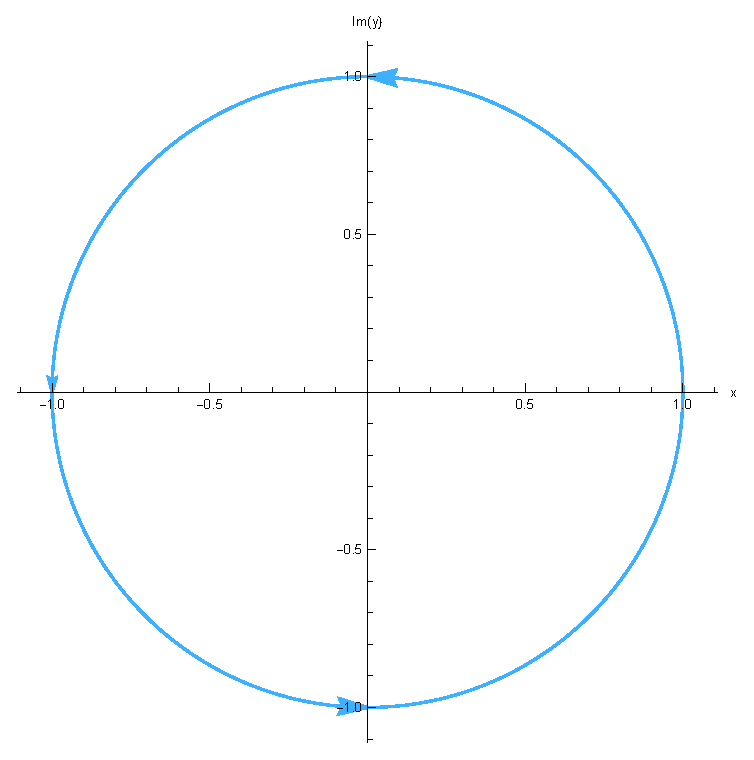
\includegraphics[scale = 0.7]{./figs/chapter_2/curve_ex_2.eps}
            \caption{The curve $z(\theta)$ as defined above.}
        \end{figure}
\end{enumerate}
It is essential to take note of the direction of the curve. This observation will become paramount in the discussion that is to follow. For the meantime,  it is also worth noting that \textit{Lagrange's Mean Value} theorem does not hold for curves as defined above.
\begin{thm}[Invalid Lagrange' Mean Value Theorem]
    Suppose that $w(t) = u(t), iv(t)$ is a continuous curve for $t \in [a, b],$ i.e. $u(t)$ and $v(t)$ are continuous functions of $t$ in $[a, b]$. Even if $w'(t)$ exists, Lagrange's Mean Value theorem does not hold.
\end{thm}
\begin{proof}
    We need only provide a counter example. Namely,
    \[
        w(t) = e^{it}, 0 \leq t \leq 2\pi.
    \]
    In this case,
    \begin{align*}
        \frac{w(2\pi) - w(0)}{2\pi}
            &=
                0 \\
            &\neq
                w'(t), \;\forall\; t \in [0, 2\pi].
    \end{align*}
    This follows from the fact that $\abs{w'(t)} = 1, \;\forall\; t \in [0, 2\pi].$
\end{proof}

We are finally ready to define the contour integral. 

\begin{defn}[Contour Integral]
    Let $f: X \subseteq \mathbb{C} \rightarrow \mathbb{C}$ be a complex function defined for all points on the contour $C$ parametrised as $z(t) = x(t) + iy(t), t \in [a, b] \in \mathbb{R}.$ Then, the integral of $f$ over $C$ is defined as
    \[
        \int_{C} f(z)\,dz := \lim_{\norm{P} \rightarrow 0} \sum_{k = 1}^{n}f(z^{*}_{k})\Delta z_{k},
    \]
    where $P$ is a partition of the interval $[a, b]$ into $n$ distinct parts into subintervals $[t_{k - 1}, t_{k}], k \in [0, n]$ where $\Delta t_{k} = t_{k} - t_{k - 1}.$ This gives us that $\Delta z_{k} := z_{k} - z_{k - 1} := z(t_{k}) - z(t_{k - 1}).$ Finally, $z^{*}_{k}$ is a random point on $C$ in the subinterval $[t_{k - 1}, t_{k}].$
\end{defn}
A caveat is that the integral is meaningful when the limit exists. For this to be true, we must at least have that $f$ is continuous and $C$ is smooth or atleast piecewise smooth. This definition, is akin to that of the Riemann Integral in the real setting. To begin our examples and see the Contour integral in action, we first see how complex functions with real domains can be integrated. We will practically define the contour integral after this (as for  now, the defintion insinuates that we must divide a given contour into an infinte number of pieces which is by no means parctical). In this case, the real and imaginaary parts can be seperated or $i$ can be treated as a constant during the familiar Riemann integration. If we have a complex valued function, with a real domain defined as $f(t) = x(t) + iy(t), t \in [a, b],$ then
\begin{align*}
    \int_{a}^{b} f(t)\,dt
        &=
            \int_{a}^{b} x(t)\,dt + i\int_{a}^{b} v(t)\,dt \\
        &=
            \int_{a}^{b} \Re f(t)\,dt + i\int_{a}^{b} \Im f(t)\,dy.
\end{align*}
Which means that 
\begin{align*}
    \Re \int_{a}^{b} f(t)\,dt
        &= 
            \int_{a}^{b} \Re f(t)\,dt. \\
    \Im \int_{a}^{b} f(t)\,dt
        &= 
            \int_{a}^{b} \Im f(t)\,dt.
\end{align*}

\begin{exmp}
    $f(t) = e^{it}, t \in [0, \pi / 4].$
\end{exmp}
\begin{align*}
    \int_{a}^{b} f(t)\,dt
        &=
            \int_{0}^{\pi / 4} e^{it}\,dt \\
        &=
            \frac{1}{i}
            \left[
                e^{it}
            \right]_{0}^{\pi / 2} \\
        &=
            \frac{1}{\sqrt{2}} + i\left(1 - \frac{1}{\sqrt{2}}\right)
\end{align*}

\begin{exmp}
    $f(t) = e^{(1 + i)x}, x \in [0, \pi].$
\end{exmp}
\[
    \int_{a}^{b} f(x)\,dx = \int_{0}^{\pi} e^{x}\cos x\,dx + i\int_{0}^{\pi} e^{x}\sin x\,dx.
\]
Therefore,
\[
    \int_{0}^{\pi} e^{x}\cos x\,dx = -\frac{1}{2}(1 + e^{\pi})
\]
and
\[
    \int_{0}^{\pi} e^{x}\sin x\,dx = \frac{1}{2}(1 + e^{\pi}).
\]
Which gives us that 
\[
    \int_{0}^{\pi} e^{(1 + i)x}\,dx = -\frac{1}{2}(1 + e^{\pi}) + \frac{i}{2}(1 + e^{\pi}).
\]

It is certainly the case that in functions in the examples above, the properties of the Riemann integral (such as linearity) hold. It is an important question to pose, as to whether the parametrisation of a curve is unique and the consequence of this on the contour integral itself. To take a step towards our final destination, we first prove the following theorem. It is easy to see that the parametric representation of the arc is not unique using the following example
\begin{align*}
    z(t) &= e^{it}, t \in [0, 2\pi], \\
    z(t) &= \frac{2t}{1 + t^2} + i\frac{1 - t^2}{1 + t^2},
\end{align*}
however, both defintions lead to the same arc in the plane and infact, they have the same length (which should be obvious but is stated explicitly below).

\begin{thm}[Length Preservation]
    Let $C: z(t), t \in [a, b]$ be a contour parametrised by $t \in \mathbb{R}.$ Then, if $t := \phi(\tau), \tau \in [\alpha, \beta],$ where both $\phi$ and $\phi'$ are continuous and $\phi'(\tau) > 0,$ then 
    \[
        \int_{a}^{b} \abs{z'(t)}\,dt = \int_{\alpha}^{\beta} (z(\phi(\tau)))'\,d\tau.
    \]
\end{thm}
\begin{proof}
    If $z(t) = x(t) + iy(t),$ then
    \begin{align*}
        &&z(t) 
            &=
                x(t) + iy(t) \\
        &\Rightarrow &z(\phi(\tau)) 
            &= 
                x(\phi(\tau)) + iy(\phi(\tau)) \\
        &\Rightarrow &z(\phi(\tau))'
            &=
                [x'(\phi(\tau)) + y'(\phi(\tau))]\phi'(\tau) \\
        &\Rightarrow &z(\phi(\tau))'
            &=
                z'(\phi(\tau))\phi'(\tau), \\
    \end{align*}
    where $\alpha \leq \tau \leq \beta.$ We have by variable substitution and above,
    \begin{align*}
        \int_{a}^{b} \abs{z'(t)}\,dt
            &=
                \int_{\alpha}^{\beta} \abs{z'(\phi(\tau))\phi'(\tau)}\,d\tau. \\
            &=
                \int_{\alpha}^{\beta} \abs{z(\phi(\tau))'}\,d\tau. \\
    \end{align*}
\end{proof}
The above theorem was important because of the discussion that is about to follow. In essence, it was to verify the practical defintion (below) of the contour intgral and make sure that it is well defined. We state the (practical) definiton of the complex contour integral as a theorem. 
\begin{thm}[Contour Integral]
    Let $f: X \subseteq \mathbb{C} \rightarrow \mathbb{C}$ be a complex function defined for all points on the contour $C$ parametrised as $z(t) = x(t) + iy(t), t \in [a, b] \in \mathbb{R}.$ Then,
    \[
        \int_{C} f(z)\,dz = \int_{a}^{b} f(z(t))z'(t)\,dt.
    \]
\end{thm}
\begin{proof}
    If we consider, the contour integral as in \defnref{2.2.25}, then we can make the following subsitutions 
    \[
        f(z) = u(x(t), y(t)) + iv(x(t), y(t)), \Delta z = \Delta x(t) + i\Delta y(t).
    \]
    This gives us
    \begin{align*}
        \int_{C} f(z)\,d\Delta z \\
            &=    
                \lim_{\norm{P} \rightarrow 0} \sum_{k = 1}^{n}(u(x(t)_{k}^{*}, y(t)^{*}) + iv(x(t)_{k}^{*}, y(t)^{*}))(\Delta x(t) + i\Delta y(t)) \\
        \begin{split}
            &=
                \lim_{\norm{P} \rightarrow 0} \sum_{k = 1}^{n}u(x(t)^{*}, y(t)^{*})\Delta x(t) + i(u(x(t)^{*}, y(t)^{*})\Delta y(t) \\
            &\qquad+ 
                v(x(t)^{*}, y(t)^{*})\Delta x(t)) - v(x(t)^{*}, y(t)^{*})\Delta y(t) \\
        \end{split}
        \\
        \begin{split}
            &=
                \lim_{\norm{P} \rightarrow 0} \left[\sum_{k = 1}^{n}(u(x(t)^{*}, y(t)^{*})\Delta x(t) - v(x(t)^{*}, y(t)^{*})\Delta y(t))\right. \\
            &\qquad+ 
                i\left.\sum_{k = 1}^{n} (u(x(t)^{*}, y(t)^{*})\Delta y(t) + v(x(t)^{*}, y(t)^{*})\Delta x(t))\right] \\
        \end{split}
        \\
        \begin{split}
            &=
                \int_{C} u(x(t), y(t))\,dx(t) -v(x(t), y(t))\,dy(t) \\
            &\qquad+ 
                i\int_{C} v(x(t), y(t))\,dx(t) + u(x(t), y(t))\,dy(t) \\
        \end{split}
        \\
        \begin{split}
            &=
                \int_{a}^{b} u(x(t), y(t))x'(t)\,dt -v(x(t), y(t))y'(t)\,dt \\
            &\qquad+ 
                i\int_{a}^{b} v(x(t), y(t))x'(t)\,dt + u(x(t), y(t))y'(t)\,dt \\
        \end{split}
        \\
            &=
                \int_{a}^{b} [u(x(t), y(t)) + iv(x(t), y(t))](x'(t) + iy'(t))\,dt \\
            &=
                \int_{a}^{b} f(z(t))z'(t)\,dt.
    \end{align*}
\end{proof}

The linearity of the contour integral (as defined above) arises naturally from the linearity of the Riemann integral. Namely, if $f, g: X \subseteq \mathbb{C} \rightarrow \mathbb{C}$ be complex functions defined for all points on the contour $C$ and let $z_0 \in \mathbb{C},$ then,
\[
    \int_{C} (f(z) + z_0g(z))\,dz = \int_{C} f(z)\,dz + z_0\int_{C} g(z)\,dz.
\]

\begin{thm}[Contour Integral Orientation]
    Let $f: X \subseteq \mathbb{C} \rightarrow \mathbb{C}$ be a complex function defined for all points on the contour $C$ parametrised as $z(t) = x(t) + iy(t), t \in [a, b] \in \mathbb{R}.$ If we denote, $-C: z(-t), t \in [-b, -a],$ (as the contour with its direction reversed during construction) then
    \[
        \int_{-C} f(z)\,dz = -\int_{C} f(z)\,dz.
    \]
\end{thm}
\begin{proof}
    With the variable subsitution $u = -t,$ we have
    \begin{align*}
        \int_{-C} f(z)\,dz 
            &=
                -\int_{-b}^{-a} f(z(-t))z'(-t)\,dt \\
            &=
                -\int_{a}^{b} f(z(u))z'(u)\,du. \\
            &=
                -\int_{C} f(z)\,dz.
    \end{align*}
\end{proof}

Upto this point we have been lose with what we mean by \textit{orientation.} To make it a bit more precise, the convention used is that if curves are constructed anticlockwise then they have a positive orientation and negative if clockwise (just like angles in the plane.) To this end we further prove a theorem that allows one to deconstruct the contour integral into sub-integrals on individual contours. This is because our defintion of the contour accounted for the fact that it may be an inductively constructed object made of end to end joined smooth curves.

\begin{thm}
    Let $f: X \subseteq \mathbb{C} \rightarrow \mathbb{C}$ be a complex function defined (and continuous) for all points on the contour $C$ (piecewise smooth)) parametrised as $z(t) = x(t) + iy(t), t \in [a_{1}, b_{n}] \in \mathbb{R},$ where $C = C_1 + C_2 + \cdots + C_n$ (all smooth contours joined end to end) parametrised as $z_{k}(t) = x_{k}(t) + iy_{k}(t), t_{k} \in [a_{k}, b_{k}] \in \mathbb{R},$ where $z_{k - 1}(b_{k - 1}) = z_{k}(a_{k})$ (for all $k = 1, 2, \cdots, n$). Then,
    \[
        \int_{C} f(z)\,dz = \sum_{k = 1}^{n} \int_{C_{k}} f(z)\,dz.
    \]
\end{thm}
\begin{proof}
    We prove this theorem using induction.

    \noindent \textbf{Base case} $\mathbf{n = 2:}$ We have 
    \begin{align*}
        \int_{C} f(z)\,dz
            &=
                \int_{C_1 + C_2} f(z)\,dz \\
            &=
                \int_{a_{1}}^{b_{2}} f(z_{1}(t) + z_{2}(t))(z_{1}'(t) + z_{2}'(t))\,dt \\
            &=
                \int_{a_{1}}^{b_{1}} f(z_{1}(t) + z_{2}(t))(z_{1}'(t) + z_{2}'(t))\,dt + \int_{a_{a_2}}^{b_{2}} f(z_{1}(t) + z_{2}(t))(z_{1}'(t) + z_{2}'(t))\,dt \\
            &=
                \int_{a_{1}}^{b_{1}} f(z_{1}(t))z_{1}'(t)\,dt + \int_{a_{2}}^{b_{2}} f(z_{2}(t))z_{2}'(t)\,dt \\
            &=
                \int_{C_1} f(z)\,dz + \int_{C_2} f(z)\,dz,
    \end{align*}
    which is possible because $b_1 = a_2.$

    \noindent \textbf{Inductive hypothesis} $\mathbf{n = k:}$ We assume that the statement is true for some $k > 2.$ We then consider
    \begin{align*}
        \int_{C} f(z)\,dz
            &=
                \int_{\sum_{j = 1}^{k + 1}C_{j}} f(z)\,dz \\
            &=
                \int_{\sum_{j = 1}^{k}C_{j}} f(z)\,dz + \int_{C_{k + 1}} f(z)\,dz \\
            &=
                \int_{\sum_{j = 1}^{k - 1}C_{j}} f(z)\,dz + \int_{C_{k}} f(z)\,dz + \int_{C_{k + 1}} f(z)\,dz \\
            &= 
                \\
            & \quad\vdots 
                \\
            &=
                \sum_{j = 1}^{k + 1} \int_{C_{j}} f(z)\,dz.
    \end{align*}
    Here the subsequent removal of the last integral from the sum in each step is possible due to the base case. This closes the induction process.  
\end{proof}
It is worth noting that writing the contour $C$ (as above) as $C_1 + C_2 + \cdots + C_n$ is a convention. It should actually be $C_1 \cup C_2 \cup  \cdots \cup C_n$ because of the defintion that it is a set of points. But the notation above sits well with the fact the contour is in fact $z_{1}(t) + \cdots + z_{n}(t).$

\begin{exmp}
    \[
        \int_{C} (y - x - 3ix^2)\,dz, z = x + iy,
    \]
where $C = C_1 + C_2 + C_3$, such that $z_{1}(t) = it, z_{2}(t) = t + i, z_{3}(t) = t + it,$ $0 \leq t \leq 1.$
\end{exmp}
The contour is shown below
\begin{figure}[H]
    \centering
    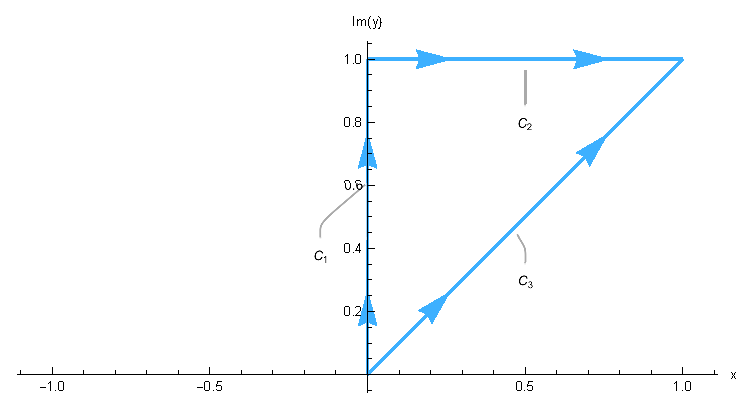
\includegraphics[scale = 0.7]{./figs/chapter_2/ci_contour_ex_1.eps}
    \caption{Contour in \exmpref{2.2.21}.}
\end{figure}

We have,

\noindent $\mathbf{C_1}:\; z(t) = it, 0 \leq t \leq 1:$ \\
\begin{align*}
    \int_{C_1} (y - x - 3ix^2)\,dz
        &=
            \int_{0}^{1} it i\,dt \\
        &=
            -\int_{0}^{1} t\,dt \\
        &=
            -\frac{1}{2}.
\end{align*}

\noindent $\mathbf{C_2}:\; z(t) = t + i, 0 \leq t \leq 1:$ \\
\begin{align*}
    \int_{C_1} (y - x - 3ix^2)\,dz
        &=
            \int_{0}^{1}  (1 - t - 3it^2)\,dt \\
        &=
            -\int_{0}^{1} t\,dt \\
        &=
            \frac{1}{2} - i.
\end{align*}

\noindent $\mathbf{C_3}:\; z(t) = t + it, 0 \leq t \leq 1:$ \\
\begin{align*}
    \int_{C_3} (y - x - 3ix^2)\,dz
        &=
            \int_{0}^{1}  (t - t - 3it^2)(1 + i)\,dt \\
        &=
            -\int_{0}^{1} t\,dt \\
        &=
            1 - i.
\end{align*}

Therefore,
\[
    \int_{C} (y - x - 3ix^2)\,dz = 1 - 2i.
\]

\begin{exmp}
    \[
        \int_{C} \overline{z}\,dz,
    \]
    where $C: z(t) = 2e^{it}, t \in [-\pi/2, \pi/2].$
\end{exmp}

\begin{align}
    \int_{C} \overline{z}\,dz \\
        &=
            \int_{-\pi/2}^{\pi/2}2e^{-it}2ie^{it}\,dt \\
        &=
            4i\int_{-\pi/2}^{\pi/2}\,dt \\
        &=
            4\pi i.
\end{align}

\begin{thm}[Constrained Integrals]
    If $C: z(t), t \in [a, b]$ is a piecewise continous contour, then 
    \[
        \abs{\int_{a}^{b} z(t)\,dt} \leq \int_{a}^{b}\abs{z(t)}\,dt. 
    \]
\end{thm}
If
\[
    \int_{a}^{b} z(t)\,dt = 0,
\]
then the inequality holds trivially.
If we assume that 
\[
    \int_{a}^{b} z(t)\,dt = r_0e^{i\theta_0},
\]
then
\begin{align*}
    &&r_0
        &=
            \int_{a}^{b} e^{i\theta_0}z(t)\,dt \\
    &\Rightarrow &r_0
        &=
            \Re \int_{a}^{b} e^{i\theta_0}z(t)\,dt \\ 
    &\Rightarrow &r_0
        &=
            \int_{a}^{b} \Re [e^{i\theta_0}z(t)]\,dt.
\end{align*}
Now,
\begin{align*}
    \abs{\Re [e^{i\theta_0}z(t)]}
        &\leq
            \abs{e^{i\theta_0}z(t)} \\
        &\leq
            \abs{z(t)}, \;\forall\; t \in [a, b].
\end{align*}
Therefore,
\[
    \abs{\int_{a}^{b} z(t)\,dt} = \int_{a}^{b}\abs{\Re[e^{i\theta_0}z(t)]}\,dt \leq \int_{a}^{b}\abs{z(t)}\,dt.
\]

\begin{thm}[Bounded Integrals]
    Let $C: z(t), t \in [a, b]$ be a smooth contour with length $L$ and suppose that a function $f: X \subseteq \mathbb{C} \rightarrow \mathbb{C}$ is piecewise continuous on $C.$ If $f$ is bounded in $X$, i.e.
    \[
        \exists M > 0: \abs{f(z)} \leq M, z \in X,
    \]
    then
    \[
        \abs{\int_{a}^{b} f(z)\,dt} \leq ML.
    \]
\end{thm}
\begin{proof}
    We have,
    \begin{align*}
        \abs{\int_{C}f(z)\,dz}
            &\leq
                \int_{a}^{b} \abs{f(z(t))z'(t)}\,dt \\
            &=
                \int_{a}^{b} \abs{f(z(t))}\abs{z'(t)}\,dt \\
            &\leq
                M\int_{a}^{b}\abs{z'(t)}\,dt \\
            &=
                ML.
    \end{align*}
\end{proof}

\begin{exmp}
    \[
        \abs{\int_{C} \frac{z + 4}{z^3 - 1}}\,dz \leq \frac{6\pi}{7},
    \]
    where $C: \abs{z} = 2, z = 2$ to $z = 2i.$
\end{exmp}
We have,
\begin{align*}
    \abs{z + 4} 
        &\leq \abs{z} + 4 \\
    \abs{z^3 - 1}
        &\geq \abs{\abs{z^{3}} - 1}
\end{align*}
On the contor $C$, we can bound the numerator and denominator as 
\begin{align*}
    \abs{z + 4} 
        &\leq 6 \\
    \abs{z^3 - 1}
        &\geq 7.
\end{align*}
Which means that on the contour $C$, 
\[
    \abs{\frac{z + 4}{z^3 - 1}} \leq \frac{6}{7}.
\]
The length of the contour in given by the integral
\begin{align*}
    \int_{C}\,dt
        &=
            \int_{0}^{\pi/2} \abs{z'(t)}\,dt \\
        &=
            \int_{0}^{\pi/2} 2\,dt \\
        &=
            \pi.
\end{align*}
Therefore,
\[
    \abs{\int_{C} \frac{z + 4}{z^3 - 1}}\,dz \leq \frac{6\pi}{7}.
\]

\begin{exmp}
    \[
        \lim_{R \rightarrow \infty} \int_{C_{R}} \frac{\sqrt{z}}{z^2 + 1}\,dz,
    \]
    where $C_{R}: z(\theta) = Re^{i\theta}, 0 \leq \theta \leq \pi.$
\end{exmp}
The contour integral can be written as 
\[
    \int_{0}^{\pi} \frac{\sqrt{R} e^{i(\theta / 2 + 2k\pi)}}{R^2e^{2i\theta} + 1}\,d\theta.
\]
where $k = 0, 1.$ We have the following restrictions to the numerator and denomiator on the contour $C_{R}$
\begin{align*}
    \abs{\sqrt{z}}
        &=
            \abs{\sqrt{R} e^{i(\theta / 2 + 2k\pi)}} \\
        &=
            \sqrt{R}. \\
    \text{and} \\
    \abs{z^2 + 1}
        &=
            \abs{R^2e^{2i\theta} + 1} \\
        &\geq
            R^2 - 1. \\
\end{align*}
We finally have that 
\begin{align*}
    \lim_{R \rightarrow \infty}\abs{\int_{0}^{\pi} \frac{\sqrt{R} e^{i(\theta / 2 + 2k\pi)}}{R^2e^{2i\theta} - 1}\,dt} 
        &\leq 
            \lim_{R \rightarrow \infty}\frac{\pi R\sqrt{R}}{R^2 - 1} \\
        &\rightarrow 
            0.
\end{align*}
Which implies
\[
    \lim_{R \rightarrow \infty} \int_{C_{R}} \frac{\sqrt{z}}{z^2 + 1}\,dz = 0.
\]

\begin{exmp}
    \[
        \abs{\int_{C} \frac{dz}{z^4}} \leq 4\sqrt{2},
    \]
    where $C: z(t) = t + i(1 - t), 0 \leq t \leq 1.$
\end{exmp}
The contour is shown below.
\begin{figure}[H]
    \centering
    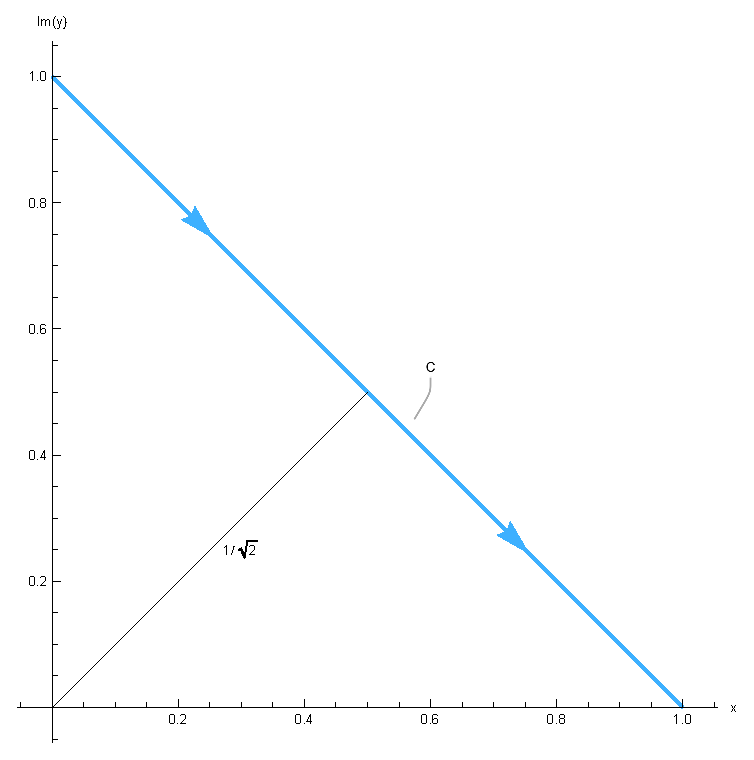
\includegraphics[scale = 0.7]{./figs/chapter_2/ci_contour_ex_2.eps}
    \caption{Contour of the function $z(t) = t + i(1 - t)$}
\end{figure}
As shown the minimum value of $\abs{z}$ is $1\sqrt{2}.$ Therefore,
\[
    \abs{z^{4}} = \abs{z}^{4} \geq \frac{1}{4}.
\]
Allowing us to infer that
\begin{align*}
    \abs{\int_{C} \frac{dz}{z^4}}
        &\leq
            \int_{C}4\,dz \\
        &\leq
            4\sqrt{2}.
\end{align*}
The length of the contour is $\sqrt{2}.$

\begin{exmp}
    \[
        \abs{\int_{C} e^z - \overline{z}\,dz} \leq 60, 
    \]
    where $C$ is the contour shown in the diagram. 
\end{exmp}
\begin{figure}[H]
    \centering
    \includegraphics[scale = 0.7]{./figs/chapter_2/ci_contour_ex_3.eps}
    \caption{Contour for \exmpref{2.2.26}.}
\end{figure}
We have, 
\begin{align*}
    \abs{e^z - \overline{z}}
        &\leq
            \abs{e^z} + \abs{\overline{z}} \\
        &=
            e^x + \abs{z} \\
        &\leq 
            5.
\end{align*}
Along the contour the maximum value of $e^x$ is 1. The length of the contour $L = 12.$ Therefore, 
    \[
        \abs{\int_{C} e^z - \overline{z}\,dz} \leq 60.
    \]

\begin{exmp}
    \[
        \abs{\int_{C_R} \frac{2z^ - 1}{z^4 + 5z^2 + 4}\,dz} \leq \frac{\pi R (2R^2 + 1)}{(R^2 - 1)(R^2 - 4)},
    \]
    where $C$ is the upper half of $\abs{z} = R, R > 2.$
\end{exmp}
On the contour, the upper bound of the numerator is 
\[
    \abs{2z^2 - 1} \leq 2\abs{z^2} + 1 = 2R^2 + 1
\]
and the lower bound of the denominator is 
\begin{align*}
    \abs{z^4 + 5z^2 + 4}
        &=
            \abs{z^2 + 4}\abs{z^2 + 1} \\
        &\leq
            \abs{\abs{z^2} -4}\abs{\abs{z^2} - 1} \\
        &=
            (R^2 - 4)(R^2 - 1).
\end{align*}
The length of the contour is $\pi R.$ This gives us the constraint 
\[
    \abs{\int_{C_R} \frac{2z^ - 1}{z^4 + 5z^2 + 4}\,dz} \leq \frac{\pi R (2R^2 + 1)}{(R^2 - 1)(R^2 - 4)}.
\]

\begin{exmp}
    Let $C_{\rho}: \abs{z} = \rho, \rho \in (0, 1)$ and $f$ be a complex valued function that is analytic in $\abs{z} \leq 1.$ Then,
    \[
        \lim_{\rho \rightarrow 0} \int_{C_{\rho}} z^{-1/2}f(z)\,dz = 0.
    \]
\end{exmp}
Since $f(z)$ is analytic for $\abs{z} \leq 1,$ it is continuous in that region and there exists $M > 0$ such that 
\[
    \abs{f(z)} \leq M, \abs{z} \leq 1.
\]
Also,
\[
    z^{-1/2} = \frac{1}{\sqrt{\rho}}e^{-i \theta / 2 + 2k\pi},
\]
where $k = 0, 1$ and $z = \rho e^{i\theta}.$ Taking the principal branch, i.e. $k = 0,$ we have
\begin{align*}
    \lim_{\rho \rightarrow 0} \abs{\int_{C_{\rho}} z^{-1/2}f(z)\,dz} 
        &\leq
            \lim_{\rho \rightarrow 0} 2\pi \rho * M / \sqrt{\rho} \\
        &=
            0.
\end{align*}
The result now follows.

\begin{exmp}
    Define the polynomial 
    \[
        P_{n}(x) = \frac{1}{\pi}\int_{0}^{\pi}(x + i \sqrt{1 - x^2}\cos\theta)^{n}\,d\theta.
    \]
    where $-1 \leq x \leq 1$ and $n \in \mathbb{N}\cup\{0\}.$ Then,
    \[
        \abs{P_{n}(x)} \leq 1.
    \]
\end{exmp}
We have,
\begin{align*}
    \abs{x + i\sqrt{1 - x^2}\cos\theta}
        &\leq
            \abs{x} + \abs{\sqrt{1 - x^2}} \\
        &leq
            1.
\end{align*}
Which follows from the fact that $\abs{x} \leq 1.$ Now,
\begin{align*}
    \abs{P_{n}(x)}
        &=
            \frac{1}{\pi}\abs{\int_{0}^{\pi}(x + i \sqrt{1 - x^2}\cos\theta)^{n}\,d\theta} \\
        &\leq
            \frac{1}{\pi}\int_{0}^{\pi}\abs{x + i \sqrt{1 - x^2}\cos\theta}^{n}\,d\theta \\
        &\leq
            \frac{1}{\pi} \int_{0}^{\pi}d\theta\\
        &=
            1.
\end{align*}
We now state a fundamental theorem of line integrals (an extension of the fundamental theorem of calculus) which we will later use extensively to prove more specialised theorems.

\begin{thm}
    Suppose that $f: X \subseteq \mathbb{C} \rightarrow \mathbb{C}$ is a continuous function on some domain $D \subseteq X.$ If anyone of the following statements is true, then so are the others
    \begin{enumerate}[label = {(\roman*)}]
        \item
            $f$ has an antiderivative $F$ throughout D.
        \item
            The integrals of $f$ along any smooth contours between two points $z_1$ and $z_2$ in $\mathbb{C}$ is $F(z_2) - F(z_1)$ assuming that the contour flows from $z_1$ to $z_2$.
        \item
            The integrals of $f$ along any closed and smooth contour lying entirely in $D$ is 0.
    \end{enumerate}
\end{thm}
\begin{proof}
    (i) $\Rightarrow$ (ii)
    Assume that $f$ has an antiderivative $F$ in $D$. Let $C: z(t), t \in [a , b]$ be a contour lying in $D$ such that $z(a) = z_1$ and $z(b) = z_2.$ Then, 
    \[
        \frac{d}{dt} F(z(t)) = F'(z(t))z'(t) = f(z(t))z'(t)
    \]
    and
    \begin{align*}
        \int_{C} f(z)\,dz
            &=
                \int_{a}^{b} f(z(t))z'(t)\,d(t) \\
            &=
                \int_{a}^{b} \frac{d}{dt}F(z(t))\,dt \\
            &=
                F(z(b)) - F(z(a)).
    \end{align*}
    
    \noindent (ii) $\Rightarrow$ (iii)
    Suppose that 
    \[
        \int_{C} f(z)\,dz = F(z_2) - F(z_1),
    \]
    where $C$ is a smooth contour lying in $D$, extending from $z_1$ to $z_2$. Then, we let $z_1$ and $z_2$ lie on a closed contour $C$ in $D.$ Then, there can be two paths that can be taken from $z_1$ to $z_2$ in $D$. One anticlockwise and the other clockwise. Let us say these paths are represented as $C_1$ and $C_2$ respectively extending between $z_1$ and $z_2$. Without loss of generality, the closed contour $C = C_1 - C_2.$ From our assumption we must have that
    \begin{align*} 
        &
            &\int_{C_{1}} f(z)\,dz 
                &=
                    \int_{C_2} f(z)\,dz \\
        &\Rightarrow 
            &\int_{C_{1}}f(z)\,dz - \int_{C_2} f(z)\,dz
                &=
                    0 \\
        &\Rightarrow 
            &\int_{C_1 - C_2} f(z)\,dz
                &=
                    0 \\
        &\Rightarrow
            &\int_{C} f(z)\,dz
                &=
                    0.
    \end{align*}
    This implies (iii).

    \noindent (iii) $\Rightarrow$ (i)
    Finally, assume that 
    \[
        \int_{C} f(z)\,dz = 0,
    \]
    where $C$ is any closed contour in $C.$ Define the integral
    \[
        F(s) := \int_{z_0}^{z}f(s)\,ds.
    \]
    Consider the small step $\Delta z$
    \begin{align*}
        F(z + \Delta z) - F(z) 
            &= 
                \int_{z_0}^{z + \Delta z}f(s)\,ds - \int_{z_0}^{z}f(s)\,ds \\
            &= 
                \int_{z}^{z + \Delta z}f(s)\,ds \\
    \end{align*}
    If we select the line segment from $z$ to $z + \Delta z,$ then
    \[
        \int_{z}^{z + \Delta z} ds = \Delta z.
    \]
    Therefore,
    \begin{align*}
        \frac{F(z + \Delta z) - F(z)}{\Delta z} - f(z)
            &=
                \frac{1}{\Delta z}\int_{z}^{z + \Delta z} f(s)\,ds - f(z) \\
            &=
                \frac{1}{\Delta z}\int_{z}^{z + \Delta z} f(s)\,ds - \frac{1}{\Delta z}\int_{z}^{z + \Delta z} f(z)\,ds \\
            &=
                \frac{1}{\Delta z}\int_{z}^{z + \Delta z} f(s) - f(z)\,ds.
    \end{align*}
    Since $f$ is continuous, at $z$, $\forall\; \epsilon > 0 \;\exists\; \delta > 0:$
    \[
        d(s, z) < \delta \Rightarrow d(f(s), f(z)) < \epsilon.
    \] 
    We may let $\abs{\Delta z} < \delta$ as it is arbitrary, then
    \[
        \abs{\frac{F(z + \Delta z)}{\Delta z} - f(z)} < \frac{1}{\abs{\Delta z}} \epsilon \Delta z = \epsilon.
    \]
    Therefore, $F'(z) = f(z)$ in $D.$ This closes the proof.
\end{proof}

\begin{exmp}
    \[\int_{0}^{1 + i} z^2\,dz\].
\end{exmp}
\begin{align*}
    \int_{0}^{1 + i} z^2\,dz
        &=
            \left[\frac{z^3}{3}\right]_{0}^{1 + i} \\
        &=
            \frac{2}{3}(-1 + i).
\end{align*}
Note that it does not matter on which contour we integrate in the interval $z = 0$ to $z = 1+ i.$

\begin{exmp}
    \[
        \int_{C} \frac{dz}{z^2},
    \]
    where $C: z(\theta) = 2e^{i\theta}, -\pi \leq \theta \leq \pi.$
\end{exmp}
Since the antiderivative of $1/z^2$ is $-1/z$ in $\mathbb{C}$, we have 
\[
    \int_{C} \frac{1}{z^{2}}\,dz = 0.
\]

\begin{exmp}
    \[
        \int_{C} \frac{dz}{z},
    \]
    where $C: z(\theta) = 2e^{i\theta}, -\pi/2 \leq \theta \leq \pi/2.$
\end{exmp}
We have that 
\[
    \frac{d}{dz}\ln z = \frac{d}{dz}[\ln\abs{z} + i(\phi + 2n\pi)] = \frac{1}{z}.
\]
where $\phi + 2n\pi = arg z,$ and $n \in \mathbb{Z}.$  Taking the principal branch, we get
\begin{align*}
    \int_{C} \frac{dz}{z}
        &=
           \left[ \ln\abs{z} + i\phi \right]_{-2i}^{2i} \\
        &=
            i\pi.
\end{align*}

\begin{exmp}
    \[
        \int_{C} z^{1/2}\,dz,
    \]
    where $C$ is any contour from $z = -3$ to $z = 3$ lying above the $x-$axis.
\end{exmp}
$z^{1/2} = \sqrt{\abs{z}}e^{i\theta / 2},$ where $\theta = Arg z.$ (the prinicipal branch). This is not defined at $z = 3,$ therefore
\[
    -\frac{\pi}{2} < \theta < \frac{\pi}{2}.
\]
The antiderivative of $z^{1/2}$ becomes 
\[
    \frac{2}{3} z^{3/2} = \frac{2}{3}\abs{z}^{3/2}e^{i3\theta/2}.
\]
This gives 
\[
    \int_{C} z^{1/2}\,dz = 2\sqrt{3}(1 + i).
\]

\begin{exmp}
    \[
        \int_{0}^{\pi + 2i} \cos\frac{z}{2}\,dz.
    \]
\end{exmp}
As discussed in the next section the complex trignometric functions $\sin$ $\cos$ and $\tan$ are well defined and can be differentiated in $\mathbb{C}.$ Therefore, 
\[
    \frac{d}{dz} 2\sin\frac{z}{2} = \cos\frac{z}{2}.
\]
This gives
\begin{align*}
    \int_{0}^{\pi + 2i} \cos\frac{z}{2}\,dz
        &=
            2\sin\left(\frac{\pi}{2} + i\right) - 0 \\
        &=
            2\sin\left(\frac{\pi}{2} + i\right).
\end{align*}

We now state a fundamental theorem for contour integrals.
\begin{thm}[Cauchy-Goursat]
    If a function $f: X \subseteq \mathbb{C} \rightarrow \mathbb{C}$ is analytic at all points interior to a simple closed contour $C,$ then
    \[
        \int_{C} f(z)\,dz = 0.
    \]
\end{thm}
\begin{proof}
    The following proof is due to \cite{Stein2003}. The first part of the proof utilises an interesting inductive process. To this end we consider a triangle in the interior of $C,$ that is positively oriented. The triangle is divided iteratively, using the midpoints of each side as shown in the figures given below.
    \begin{figure}[H]
        \centering
        \begin{subfigure}{0.30\textwidth}
            \centering
            \includegraphics[width = \textwidth]{./figs/chapter_2/sierpinski_0.eps}
            \caption{The original triangle}
        \end{subfigure}
        \qquad
        \begin{subfigure}{0.30\textwidth}
            \centering
            \includegraphics[width = \textwidth]{./figs/chapter_2/sierpinski_1.eps}
            \caption{First iteration.}
        \end{subfigure}
        \qquad
        \begin{subfigure}{0.30\textwidth}
            \centering
            \includegraphics[width = \textwidth]{./figs/chapter_2/sierpinski_2.eps}
            \caption{Second iteration.}
        \end{subfigure}
        \caption{Successive divisions of the triangle inside the domain defined by the contour $C.$}
    \end{figure}
    {\color{red} TODO: Complete proof}
\end{proof}

The above theorem allows us to prove the following Cauchy-Integral theorem, which \textit{integral} to the say the least. 
\begin{thm}[Cauchy Integral Formula]
    Let $f: X \subseteq \mathbb{C} \rightarrow \mathbb{C}$ be analytic everywhere inside a simple closed contour $C,$ positively oriented. If $z_0 \in \mathbb{C},$ is interior to the contour, then 
    \[
        f(z_0) = \frac{1}{2\pi i} \int_{C} \frac{f(z)}{z - z_0}\,dz.
    \]
\end{thm}
\begin{proof}
    Let $C_{\rho}: S(z_0, \rho)$ where $\rho$ is small enough to allow $C_{\rho} \subset C.$ This means that $\frac{f(z_0)}{z - z_0}$ is analytic between and on the contours $C$ and $C_{\rho}.$ Consider the path $\gamma,$ on which, according to the Cauchy-Goursat theorem [$\because z_0$ is interior to $\gamma$], 
    \[
        \int_{\gamma} \frac{f(z)}{z - z_0} = 0.
    \]
    This implies
    \[
        \int_{B \rightarrow A} \frac{f(z)}{z - z_0}\,dz + \int_{A \rightarrow D} \frac{f(z)}{z - z_0}\,dz + \int_{B\rightarrow C} \frac{f(z)}{z - z_0}\,dz + \int_{C \rightarrow B} \frac{f(z)}{z - z_0}\,dz = 0.
    \]
    As the point $B$ approaches $C$ (and consequently $A$ appraoches $D$), the above experssion reduces to  
    \[
        \int_{B \rightarrow A} \frac{f(z)}{z - z_0}\,dz - \int_{B \rightarrow A} \frac{f(z)}{z - z_0}\,dz + \int_{C} \frac{f(z)}{z - z_0}\,dz - \int_{C_{\rho}} \frac{f(z)}{z - z_0}\,dz = 0.
    \]
    Therefore,
    \[
        \int_{C} frac{f(z)}{z - z_0}\,dz = \int_{C_{\rho}} frac{f(z)}{z - z_0}\,dz.
    \]
    Finally, consider the value
    \begin{align*}
        \abs{\int_{C} - 2\pi i f(z_0)}
            &=
                \abs{\int_{C} \frac{f(z)}{z - z_0}\,dz - \int_{C_{\rho}}\frac{f(z_0)}{z - z_0}\,dz} \\
            &=
                \abs{\int_{C_{\rho}}\frac{f(z) - f(z_0)}{z - z_0}\,dz}.
    \end{align*}
    Now since $f$ is analytic at $z_0,$ it is continuous there and $\forall \epsilon > 0 \;\exists\; \delta > 0: d(z, z_0) < \delta \Rightarrow d(f(z), f(z_0)) < \epsilon.$ We may choose $\rho < \delta$ such that 
    \[
        \abs{\int_{C_{\rho}}\frac{f(z) - f(z_0)}{z - z_0}\,dz} \leq \frac{\epsilon}{\rho} 2\pi\rho = 2\pi \epsilon.
    \]
    Since $\epsilon > 0$ is arbitrary,
    \[
        \int_{C} \frac{f(z)}{z - z_0}\,dz = 2\pi i f(z_0).
    \]
    It is to be noted that if $C_{\rho}: z(t) = \rho e^{it} + z_0, 0 \leq t \leq 2\pi,$ then
    \[
        \int_{C_{\rho}} \frac{dz}{z - z_0} = \int_{0}^{2\pi}\frac{i\rho}{\rho e^{it}}e^{it}\,dt = 2\pi i.
    \]
\end{proof}

\begin{thm}
    Let $f: X \subseteq \mathbb{C} \rightarrow \mathbb{C}$ be analytic everywhere inside a simple closed contour $C,$ positively oriented. If $z_0 \in \mathbb{C},$ is interior to the contour, then
    \[
        \int_{C} \frac{dz}{(z - z_0)^{n + 1}} = \frac{2\pi i}{n!}\frac{d^{n}}{dz}f(z_{0}).
    \]
\end{thm}
\begin{proof}
    The following proof uses induction on $n.$ 

    \noindent \textbf{Base Case:} $\textbf{n = 1}.$ Due to  \thmref{2.2.34}, we have 
    \[
        f(z) = \frac{1}{2\pi i} \int_{C} \frac{f(s)}{s - z}\,ds.
    \]
    We define $d := \inf\{ d(s, z) : s \in C\}.$ Now, we consider 
    \begin{align*}
        \frac{f(z + \Delta z) - f(z)}{\Delta z}
            &=
                \frac{1}{2\pi i (\Delta z)} \int_{C} \frac{f(s)}{s - z - \Delta z} - \frac{f(s)}{s - z}\,ds \\
            &=
                \frac{1}{2\pi i (\Delta z)} \int_{C} \frac{f(s)\Delta z}{(s - z - \Delta z) (s - z)}\,ds, \\
    \end{align*}
    for $0 < \abs{\Delta z} < d.$ Further,
    \begin{align*}
        \abs{\frac{f(z + \Delta z) - f(z)}{\Delta z} - \frac{1}{2\pi i} \int_{C} \frac{f(s)}{(s - z)^2}\,ds}
            &=
                \abs{\frac{1}{2\pi i} \int_{C} \frac{f(s) \Delta z}{(s - z - \Delta z)(s - z)^2}\,ds}\\
            &\leq
                \frac{L}{2\pi} \frac{\abs{\Delta z}M}{(d - \abs{\Delta z})d^2},
    \end{align*}
    where we have used the fact that $\exists \; M > 0: \abs{f(s)} < M, \forall s \;\text{on}\; C$ (because $f$ is analytic in and on $C$) and the that $\abs{s - z - \Delta z} \geq \abs{\abs{s - z} - \abs{\Delta{z}}} \geq d - \abs{\Delta z}$. Also, $L$ is the length of the contour. Now, as $\Delta z \rightarrow 0$
    \[
        \frac{f(z + \Delta z) - f(z)}{\Delta z} \rightarrow \frac{1}{2\pi i} \int_{C} \frac{f(s)}{(s - z)^2}\,ds.
    \]
    The same arguments hold for $n = k + 1,$ where the statement is assumed to be true for $n = k$ for some $k \in \mathbb{N}.$ By the principle of mathematical induction, the proof ends here. \\
    {\color{red} TODO: More detail in proof.} 
\end{proof}

\begin{exmp}
    \[
        \int_{C} \frac{1}{z^4}\,dz,
    \]
    where $C: \abs{z} = 1.$
\end{exmp}
The integral evaluates to 
\[
    \frac{2\pi i}{3!} \left.\frac{d}{dz}\right\rvert_{z = 0}\frac{1}{z^4} = \frac{8}{3} \pi i.
\]



\section{Special Functions}
\subsection{Exponential}
The exponential function as defined on the real line can be defined for complex arguments. 
\begin{defn}[Complex Expnential]
    Let $z = x + iy \in \mathbb{C}.$ Then,
    \[
        e^{z} := e^{x}e^{iy}.
    \]
\end{defn}
Familiar rules of exponents hold for example 
\begin{thm}[Exponential Rules]
    Let $z_1, z_2 \in \mathbb{C},$ where $z_1 = x_1 + iy_1$ and $z_2 = x_2 + iy_2$. Then,
    \[
        e^{z_1 + z_2} = e^{z_1}e^{z_2}.
    \]
\end{thm}
\begin{proof}
    We have,
    \begin{align*}
        e^{z_1 + z_2}
            &=
                e^{x_1 + iy_1 + x_2 + iy_2}\\
            &=
                e^{x_1 + x_2 + i(y_1 + y_2)}\\
            &=
                e^{x_1 + x_2}e^{i(y_1 + y_2)}\\
            &=
                e^{z_1}e^{z_2}.
    \end{align*}
\end{proof}
Similarly, other rules can be derived for the exponential function. It is interesting to note that the derivative of the exponential function is itself just as in the real case and the fact that a complex exponential can be negative. 
\begin{thm}[Exponential Derivative]
    If $z \in \mathbb{C},$ then
    \[
        \frac{d e^{z}}{d z} = e^{z}.
    \]
\end{thm}
\begin{proof}
    Let $p \in \mathbb{C}.$ We have that,
    \[
        e^{z} = e^{x}\cos y + ie^{x}\sin y
    \]
    Which means that $u(x, y) = e^{x}\cos y$ and $v(x, y) = e^{x}\sin y$. The partial derivatives are
    \[
        \begin{array}{cc}
            \frac{\partial u(x, y)}{\partial x} = e^{x}\cos y & \frac{\partial u(x, y)}{\partial y} = -e^{x}\sin y \\
            \frac{\partial v(x, y)}{\partial x} = e^{x}\sin y & \frac{\partial v(x, y)}{\partial y} = e^{x}\cos y.
        \end{array}
    \]
    Which are continuous in $\mathbb{R}^{2}$ and satisfy the Cauchy-Riemann equations. This means that $e^{z}$ is analytic in $\mathbb{C}$ (entire). Therefore,
    \begin{align*}
        \frac{d e^{z}}{d z}
            &=
               \frac{\partial u(x, y)}{\partial x} + i \frac{\partial v(x, y)}{\partial x} \\
            &= 
                e^{x}\cos y + ie^{x} \sin y\\
            &=
                e^{x}e^{iy} \\
            &=
                e^{z}.
    \end{align*}
\end{proof}

\begin{exmp}
    $e^{z} = i + 1$ for $z = x + iy \in \mathbb{C}$.
\end{exmp}
\begin{align*}
    &&e^{z}
        &=
            i + 1 \\
    &\Rightarrow &e^{x}e^{iy}
        &=
            i + 1 \\
    &\Rightarrow &e^{x}e^{iy}
        &=
            \sqrt{2}e^{i\pi/4} \\
    &\Rightarrow &z
        &=
            \ln \sqrt{2} + i \left(\frac{\pi}{4} + 2n\pi\right),
\end{align*}
where $n \in \mathbb{Z}.$

\begin{exmp}
    $e^{2 \pm 3i\pi} = -e^{2}.$
\end{exmp}

\begin{exmp}
    $f(z) = 2z^2 - ze^{z} + e^{-z} - 3, z \in \mathbb{C}.$
\end{exmp}
$f$ is entire because it is a combination of the entire functions $e^{z}, e^{-z}, z, 3$.

\begin{exmp} 
    $f(z) = e^{\overline{z}}, z \in \mathbb{C}$ is not analytic anywhere in $\mathbb{C}.$
\end{exmp}
We can see that 
\[
    f(x, y) = e^{x}\cos y - ie^{x}\sin y.
\]
Therefore, $u(x, y) = e^{x}\cos y$ and $v(x, y) = -e^{x}\sin y$. The partial derivatives are
\[
    \begin{array}{cc}
        \frac{\partial u(x, y)}{\partial x} = e^{x}\cos y & \frac{\partial u(x, y)}{\partial y} = -e^{x}\sin y \\
        \frac{\partial v(x, y)}{\partial x} = -e^{x}\sin y & \frac{\partial v(x, y)}{\partial y} = -e^{x}\cos y.
    \end{array}
\]
If $f$ was differentiable everywhere, we would have 
\begin{align*}
    &&\frac{\partial u(x, y)}{\partial x}
        &= 
            \frac{\partial v(x, y)}{\partial y} \\
    &\Rightarrow &\cos y 
        &=
            0 \\
    &\Rightarrow &y 
        &= 
            \frac{\pi}{2} + 2n\pi, n \in \mathbb{Z}
\end{align*}
and 
\begin{align*}
    &&\frac{\partial u(x, y)}{\partial y}
        &= 
            -\frac{\partial v(x, y)}{\partial x} \\
    &\Rightarrow &\sin y 
        &=
            0 \\
    &\Rightarrow &y 
        &= 
            2n\pi, n \in \mathbb{Z},
\end{align*}
which is not possible. Hence (by an implicit contradiction), $f$ is not analytic anywhere.

\begin{exmp}
    $\abs{e^{2z + i} + e^{iz^2}} \leq e^{2x} + e^{-2xy}, z = x + iy \in \mathbb{C}.$
\end{exmp}
\begin{align*}
    e^{2z + i}  
        &= 
            e^{2x + i(2y + 1)}
        = 
            e^{2x}e^{i(2y + 1)}, \\
    e^{iz^2}
        &=
            e^{i(x^2 - y^2 + 2ixy)}
        =
            e^{-2xy}e^{i(x^2 - y^2)}.\\   
\end{align*}
$\therefore$
\begin{align*}
    \abs{e^{2z + i} + e^{iz^2}}
        &\leq
            \abs{e^{2z + i}} + \abs{e^{iz^2}} \\
        &=
            \abs{e^{2x}e^{i(2y + 1)}} + \abs{e^{-2xy}e^{i(x^2 - y^2)}} \\
        &=
            e^{2x} + e^{-2xy}.
\end{align*}

\begin{exmp}
    $\abs{e^{z^2}} \leq e^{\abs{z}^2}, z = x + iy \in \mathbb{C}$ 
\end{exmp}
We have that 
\begin{align*}
    &&x^2 - y^2 
        &\leq 
            x^2 + y^2 \\
    &\Rightarrow &e^{x^2 - y^2}
        &\leq
            e^{x^2 + y^2} \\
    &\Rightarrow &\abs{e^{z^{2}}}
        &\leq
            e^{\abs{z}^2}.
\end{align*}

\begin{exmp}
    $e^{z} = -2, z \in \mathbb{C}.$
\end{exmp}
We have,
\begin{align*}
    &&e^{z}
        &=
            -2 \\
    &\Rightarrow &e^{z}
        &=
            2e^{i\pi} \\
    &\Rightarrow &e^{x}
        &= 
            2\;
    \text{and}\;
    y
        =
            \pi + 2n\pi, n \in \mathbb{Z}. \\
    &\Rightarrow &z
        &= 
            \ln 2 + i(\pi + 2n\pi).
\end{align*}

\begin{exmp}
    $e^{z} = 1 + \sqrt{3}i.$
\end{exmp}
\begin{align*}
    &&e^{z}
        &=
            1 + \sqrt{3}i \\
    &\Rightarrow &e^{z}
        &=
            2e^{i\pi/3} \\
    &\Rightarrow &z
        &=
            \ln 2 + i\left(\frac{\pi}{3} + 2n\pi\right), n \in \mathbb{Z}.
\end{align*}

\begin{exmp}
    $e^{2z - 1} = 1, z \in \mathbb{C}.$
\end{exmp}
\begin{align*}
    &&e^{2z - 1}
        &=
            1 \\
    &\Rightarrow &e^{2z - 1}
        &=
            e^{i0} \\
    &\Rightarrow &e^{2x - 1}e^{2iy}
        &=
            e^{i0} \\
    &\Rightarrow &e^{2x - 1}
        &=
            e^{0}\;
    \text{and}\;
    e^{2iy}
        =
            e^{i0} \\
    &\Rightarrow &z
        &=
            \frac{1}{2} + in\pi, n \in \mathbb{Z}. 
\end{align*}

\begin{exmp}
    $\overline{e^{iz}} = e^{i\overline{z}},\; \text{iff}\; z = n\pi, n \in \mathbb{Z}.$
\end{exmp}
\begin{align*}
    &&\overline{e^{iz}} 
        &= 
            e^{i\overline{z}} \\
    &\iff &\overline{e^{-y}e^{ix}}
        &=
            e^{y}e^{ix} \\
    &\iff &e^{-y}e^{-ix}
        &=
            e^{y}e^{ix} \\
    &\iff &y
        &=
            0\;
    \text{and}\;
    x
        =
            n\pi, n \in \mathbb{Z} \\
    &\iff &z
        &= 
            n\pi, n \in \mathbb{Z}.    
\end{align*}

\subsection{Logarithmic}
\begin{defn}[Complex Logarithm]
    Let $z = x + iy \in \mathbb{C}.$ Then,
    \[
        \ln z := \ln \abs{z} + i (\phi + 2n\pi), n \in \mathbb{Z},
    \]
    where $\phi = k Arg(z), k \in \mathbb{Z}.$ 
\end{defn}
The above definition maybe stated as a theorem, which arises arises naturally as a consequence of the definition of complex exponential. The question we are asking is to find $\ln z.$ This can be translated to the following, 
\[
    e^{w} = z,
\]
where $w \in \mathbb{C}.$ As we have seen in the examples above, we can use the propoerties of the exponential to solve such an equation.
If $w = u + iv$ and $z = re^{i\phi}$ then 
\begin{align*}
    &&e^{w} 
        &= 
            z \\
    &\Rightarrow &e^{u}e^{iv}
        &=
            re^{i\phi} \\
    &\Rightarrow &e^{u}
        &=
            r\;
    \text{and}\;
    e^{iv}
        =
            e^{i\phi} \\
    &\Rightarrow &w 
        &= 
            \ln r + i(\phi + 2n\pi), n \in \mathbb{Z}.
\end{align*}
Of course this definiton can be extended to logarithm of any base, and the same argument as above works in deriving that equations which is why we continue with the natural logarithm. It is important to note that $\phi$ (as above) can be any integer multiple of the argument of the complex number under consideration. It is simpler most of the times to just use the argument itself. 

\begin{exmp}
    $z = -1 - i\sqrt{3}.$
\end{exmp}
\[
    \ln z = \ln 2 + i\left(-\frac{2\pi}{3} + 2n\pi\right), n \in \mathbb{Z}.
\]

\begin{exmp}
    $\ln(-1).$
\end{exmp}
Since $-1 = e^{i\pi},$ we have
\[
    \ln(-1) = i\pi\left(1 + 2n\right), n \in \mathbb{Z}.
\]

At this juncture, it might be constructive to introduce some commonly used notation. Although, the general notion is introduced later, we take a small diversion to define the principal branch of the complex logarithm.
\begin{defn}
   The principal branch of the complex logarithm is the branch of the complex logarithm with argument $\phi$ such that the complex logarithm $\ln 1 = 0.$ It is denoted as 
   \[
        \Ln z = \ln \abs{z} + i\phi.
    \]
\end{defn}

\begin{exmp}
    $\Ln (-ei).$
\end{exmp}
\[
    \ln (-ei) = 1 + i\left(-\frac{\pi}{2} + 2n\pi\right), n \in \mathbb{Z}.
\]
Therefore, 
\[
    \Ln (-ei) = 1 - i\frac{\pi}{2}.
\]

\begin{exmp}
    $\Ln (1 - i).$
\end{exmp}
We can write $1 - i = \frac{1}{\sqrt{2}} e^{-i\pi / 4}.$ Then,
\begin{align*}
    &&\ln (1 -  i) 
        &= 
            -\frac{1}{2}\ln 2  + i\left(\frac{\pi}{4} + 2n\pi\right), n \in \mathbb{Z} \\
    &\Rightarrow &\Ln (1 - i)
        &=
            -\frac{1}{2}\ln 2  + i\frac{\pi}{4}. \\
\end{align*}

\begin{exmp}
    $\ln i.$
\end{exmp}

\begin{align*}
    &&\ln i 
        &= 
            \ln 1 + i\left(\frac{\pi}{2} + 2n\pi\right) \\
    &\Rightarrow &\ln i
        &=
        i\left(\frac{\pi}{2} + 2n\pi\right),
\end{align*}
$n \in \mathbb{Z}.$

Below we prove one familiar rule of the logarithm as seen in the real numbers. 
\begin{thm}[Log Power]
    Let $z \in \mathbb{C}$ and $n \in \mathbb{Z}.$ Then, 
    \[
        \ln z^n = n\ln z.
    \]
\end{thm}
\begin{proof}
    Let $w = \ln z^n, n \in \mathbb{Z}.$ Then, $e^{w} = z^{n}.$ We can write $z$ in polar form as $z = r\;e^{i\phi}.$ Then, by \textit{De Moivre's} theorem,
    \begin{align*}
        &&\ln z^n 
            &= 
                \ln r^{n} + i \left(n\phi + 2k\pi\right)\\ 
        &\Rightarrow &\ln z^{n}
            &=
                n (\ln r +  i\left(\phi + 2k\pi\right)\\
        &\Rightarrow &\ln z^{n}
            &=
                n \ln z.
    \end{align*}
This argument can be extended to the rationals again using the extension to \textit{De Moivre's} theorem.
\end{proof}

\begin{exmp}
    $\log_{\pi/2}(1 + i).$
\end{exmp}
\[
    \log_{\pi/2}(1 + i) = \frac{1}{2}\log_{\pi / 2} 2  + i\left(\frac{\pi}{4} + 2n\pi\right).
\]

\subsection{Trigonometric}
Euler's formula will be paramount in providing defintions of complex trigonometric functions. Assuming we know that \textit{Euler's Formula} holds for the real numbers, we can use it to define the complex trigonometric functions. Our work is a little easy as we have already defined the complex exponential.
\begin{defn}[Complex Trigonometric Functions]
    For $z \in \mathbb{C}, $ we define the following functions
    \[
        \sin z = \frac{e^{iz} - e^{-iz}}{2i}
        \;\text{and}\;
        \cos z = \frac{e^{iz} + e^{-iz}}{2}.
    \]
    This comes from adding and subtracting Euler's formula for $e^{iz}.$
\end{defn}
The complex arguments for the trigonometric functions are well posed as the right hand side of the defintions are well defined for complex values. There are other ways of defining these functions namely using the Maclaurin series expansions of the sine and cosine in the real domain and the corresponding hyporbolic trigonometric functions.

It is in fact the case that the derivatives of complex trignometric functions obey the same equations as that of the real case. We know that $e^{z}, z \in \mathbb{C}$ is entire. We can therefore use this fact to derive the derivatives of all the trigonometric functions. One such example is shown below.

\begin{thm}[Complex trigonometric derivative]
    Let $z \in \mathbb{C}.$ Then,
    \[
        \frac{d}{dz} \cos z = -\sin z.
    \]
\end{thm}
\begin{proof}
    \begin{align*}
        \frac{d}{dz} \cos z
            &=
                \frac{d}{dz} \frac{e^{iz} + e^{-iz}}{2} \\
            &=
                \frac{ie^{z} - ie^{-iz}}{2} \\
            &=
                - \frac{ie^{z} - ie^{-iz}}{2i} \\
            &=
                - \sin z.
    \end{align*}
\end{proof}

First it might be useful to note that the $\sin$ function remains odd for all complex arguments.

\begin{thm}
    Let $z \in \mathbb{C}.$ Then,
    \[
        \sin(-z) = -\sin z.
    \]
\end{thm}
\begin{proof}
    \begin{align*}
        \sin(-z)
            &=
                \frac{e^{-iz} - e^{iz}}{2i} \\
            &=
                - \frac{e^{iz} - e^{-iz}}{2i} \\
            &=
                - \sin z.
    \end{align*}
\end{proof}

We now see some of the familiar properties of trigonometric functions.

\begin{exmp}
    $\sin(z_1 + z_ 2) = \sin z_1 \cos z_2 + \sin z_2 \cos z_1, z_1, z_2 \in \mathbb{C}.$
\end{exmp}

\begin{align*}
    e^{i(z_1 + z_2)}
        &=
            e^{iz_1} e^{iz_2} \\
        &=
            (\cos z_1 + i\sin z_1) (\cos z_2 + i\sin z_2) \\
        &=
            \cos z_1 \cos z_2 - \sin z_1 \sin z_2+ i(\sin z_1 \cos z_2 + \cos z_1 \sin z_2).
\end{align*}
Comparing both sides of the equation, yields the identity above (and the identity involving $\cos(z_1 + z_2).$)

\begin{exmp}
    $\sin^{2}z + \cos^{2}z = 1, z \in \mathbb{C}.$
\end{exmp}
\begin{align*}
    1
        &=
            \cos(z - z) \\
        &=
            \cos z \cos z - \sin z \sin (-z) \\
        &=
            \cos^{2}z + \sin^{2}z.
\end{align*}

\begin{exmp}
    $\abs{\sin z}^{2} \geq \abs{\sin x}^{2},$ where $z = x + iy \in \mathbb{C}.$
\end{exmp}
We first breakdown $\sin z$ as follows
\begin{align*}
    \sin z
        &=
            \frac{e^{i(x + iy)} - e^{-i(x + iy)}}{2i} \\
        &=
            \frac{e^{-y}}{2i}(\cos x + i \sin x) - \frac{e^{y}}{2i}(\cos x - i \sin x) \\
        &=
            \left(\frac{e^{y} + e^{-y}}{2}\right)\sin x + i \left(\frac{e^{-y} - e^{y}}{2}\right)\cos x.
\end{align*}
\begin{align*}
    \abs{\sin z}^{2}
        &=
            \frac{1}{4}\left(2 \sin^{2}x - 2\cos^{2}x + e^{-2y} + e^{2y}\right) \\
        &=
            \left(\frac{\sin^{2}x}{2} - \frac{\cos^{2}x}{2} + \frac{e^{-2y} + e^{2y}}{4}\right) \\
        &=
            \sin^{2}x + \left[\frac{e^{2y} + e^{-2y}}{4} - \frac{1}{2}\right] \\
        &\geq
            \sin^{2}x.
\end{align*}
This is because the term $\frac{e^{2y} + e^{-2y}}{4} - \frac{1}{2} \geq 0,$ (simple to verify) for any $y \in \mathbb{R}.$ The conclusion now follows.

\begin{exmp}
    $\sin i\overline{z} = \overline{\sin iz} \iff z = ni\pi, n \in \mathbb{Z}, z \in \mathbb{C}.$
\end{exmp}
We have the following defintions for the hyperbolic trigonometric functions (in the real case),
\[
    \sinh x := \frac{e^{x} - e^{-x}}{2}
\]
and
\[
    \cosh x := \frac{e^{x} + e^{-x}}{2},
\]
where $x \in \mathbb{R}.$ Note that using these definitions \exmpref{2.3.19}, would have had much simpler notation. In any case, to make our task easier we will use the definitions above to expand as follows (the expansion formulas follow from \exmpref{2.3.17})
\begin{align*}
    \overline{\sin iz}
        &=
            \overline{\sin (ix - y)} \\
        &=
            \overline{\sin (-y)\cosh x + i \cos(-y)\sinh x} \\
        &=
            -\sin y \cosh x - i \cos y \sinh x.
\end{align*}
and
\begin{align*}
    \sin \overline{iz}
        &=
            \sin x\cosh y + i \cosh x\sin y \\
        &=
            \sin (-y)\cosh x + i \cos(-y)\sinh x \\
\end{align*}
Since these two quantities are considered equal, we have
\begin{align*}
    &\iff   &\sin y \cosh x &=  0       &\text{and}&     &\cos y \sinh x &= 0     \\
    &\iff   &\sin y         &=  0       &\text{and}&     &\sinh x        &= 0     \\
    &\iff   &y              &=  n\pi    &\text{and}&     &x              &= 0.
\end{align*}

\begin{exmp}
    $\sin z = \sinh 4.$
\end{exmp}
\begin{align*}
    &&\sin z 
        &= \cosh 4 \\
    &\Rightarrow &\sinh y\cos x + i \cosh y\sin x
        &= 
            \cosh 4 \\
\end{align*}
Therefore,
\[
    \cosh y\sin x  = 0 \;\text{and}\; \sinh y\cos x = \cosh 4.
\]
The first thing to notice is that $y \neq 0 \;\because\; \sin x \neq \cosh 4, \;\forall\; x \in \mathbb{R}.$ This means that $\cos x = 0.$ Which gives us
\begin{align*}
    x
        &=
            \frac{\pi}{2} + n\pi, \\
    y
        &=
            \pm 4,
\end{align*}
where $n \in \mathbb{Z}.$ Finally,
\[
    z = \frac{\pi}{2} + n\pi \pm 4i. 
\]

\begin{exmp}
    $w = \sin z, z = x + iy \in \mathbb{C}.$
\end{exmp}
In this example, we see the mapping as defined above. As in \textit{section 2.1}, we visualise the $uv$ and $xy$ planes. To mathematically get the transformation we first define some bounds, namely $\pi / 2 < x < \pi / 2$ and $-\infty < y < \infty.$ These bounds are completely arbitrary. If $x = a$ (a vertical line in the $xy-$ plane) for now assuming that $a \neq 0$, then by our nifty expansions from \exmpref{2.3.20}, we have that 
\[
    u = \sin a \cosh y \;\text{and}\; v = \cos a \sinh y, 
\]
where $u(x, y) = \sin x \cosh y$ and $v(x, y) = \cos x \sinh y$ for $(x, y) \mathbb{R}^{2}$. Since we wish to see the effect of the mapping on $x = a$, we eliminate $y,$ by using the identity
\[
    \cosh^{2} \theta - \sinh^{2} \theta = 1, \theta \in \mathbb{R}.
\]
This gives us 
\[
    \left(\frac{u}{\sin a}\right)^{2} - \left(\frac{v}{\cos a}\right)^{2} = 1,
\]
which is a parabola paramtrised by $a.$

\begin{figure}[H]
    \centering
    \begin{subfigure}{0.45\textwidth}
        \centering
        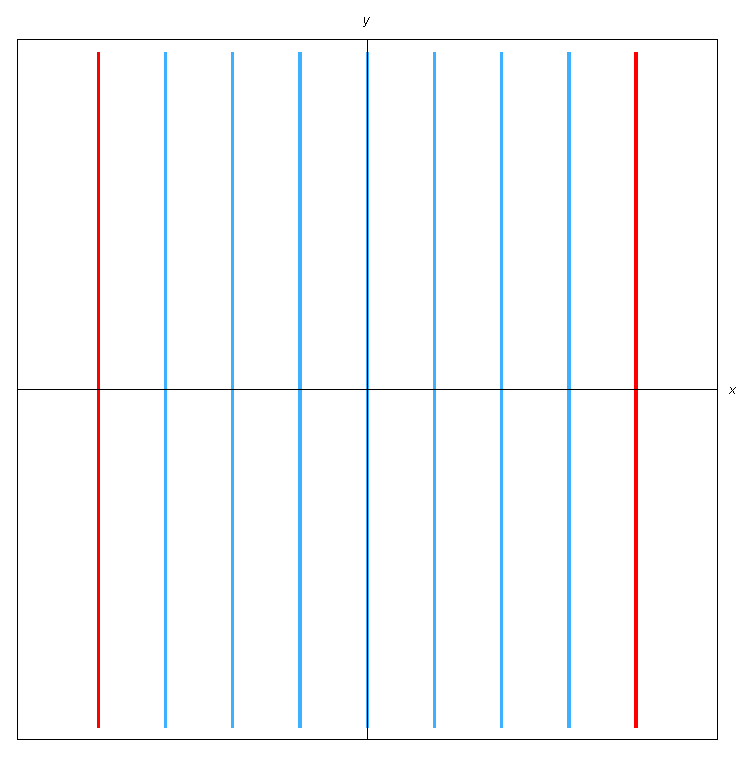
\includegraphics[width = \textwidth]{./figs/chapter_2/sin_map_z.eps}
        \caption{$xy$-plane}
    \end{subfigure}
    \qquad
    \begin{subfigure}{0.45\textwidth}
        \centering
        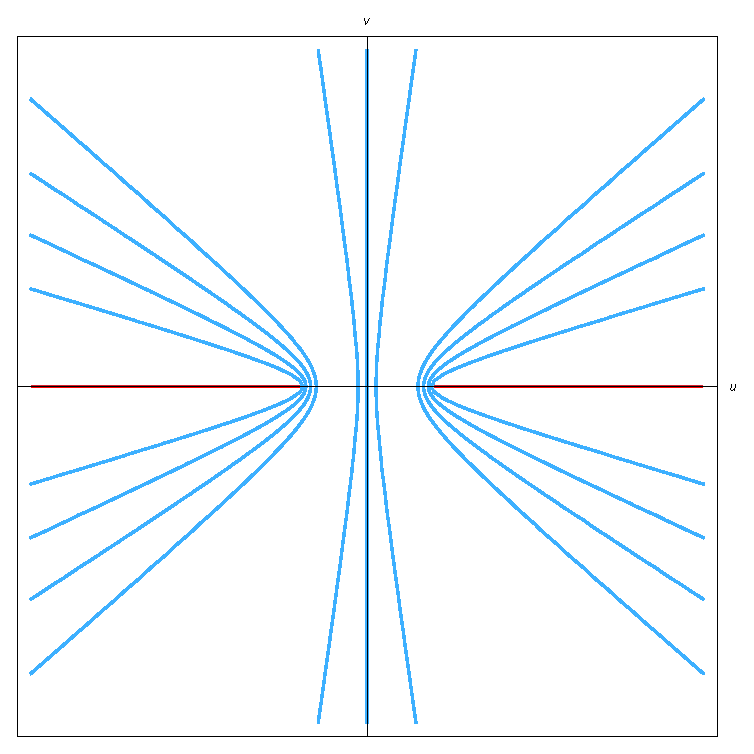
\includegraphics[width = \textwidth]{./figs/chapter_2/sin_map_w.eps}
        \caption{$uv$-plane}
    \end{subfigure}
    \caption{The light blue lines show the mapping of $x = a$ to the hyperbolas. $x = \pm \pi / 2$ is mapped to the regions $u \leq -1 \land u \geq 1,$ which are the red lines.}
\end{figure}

\cite{shanahan2003}
\printbibliography

\end{document}
